\documentclass[fleqn,12pt]{article}
\usepackage{bigpage,tech,url,javalistings,graphicx,csp-cm}
\usepackage{questions}
\def\color#1{}
\def\Programming{\textbf{[Programming]}}

\Small
%\questionsonly
\questionsandanswers
%\answersonly
%\nontuteanswersonly

\title{Concurrent Programming: Exercises}
\author{Gavin Lowe}

\sloppy

\begin{document}
\maketitle

You should complete all questions marked \Programming\ at a computer, and
include suitable testing code and test results with your answers.

Note that not all exam questions are included here.


\section{Introduction}

\input{web-browser} % Why make a web browser use concurrency?  

\begin{question}
Suppose you are designing an interactive networked application.  You decide to
have one process handling actions by the local user, and another process
handling messages that are received over the network.  What could go wrong
with this design?  Describe how you could avoid these problems.
\end{question}

\begin{answer}
There's a great danger of race conditions.  For example, suppose the
local-action-handling process executes the code \SCALA{x = x+1}, and the
network-message-handling process executes the code \SCALA{x = x-1}; as we saw
in lectures, the read and write actions of these assignments could be
interleaved in many ways, giving unintended results.

One way to deal with this problem would be to code the rest of the program as
a third process.  When either of the other two processes receives a user
action or a network message, it sends a message to the main process.  

\begin{verbatim}
 ------------------------  laChan    -----------
 | local action handler | ---------> |         |
 ------------------------            | main    |
                                     | process |
 ------------------------  nmChan    |         |
 | network msg handler  | ---------> |         |
 ------------------------            -----------
\end{verbatim}

The main process is a sequential process, which repeatedly receives a message
from one of the other threads, and acts appropriately.  Something like:
%
\begin{scala}
serve( laChan ==> { ... }
     | nmChan ==> { ... }
)
\end{scala}
%
Hence the effects of the local actions or network messages are treated
atomically.

Alternatively ---and slightly harder--- we could use a Model-View-Controller
architecture with two controllers, namely the local-action-handling and
network-message-handling processes.  The Model and View are now a separate
process, that presents various atomic operations to the controllers.  This
process again is structured as a sequential \SCALA{serve} loop, as above.
Care needs to be taken that the atomic operations can be interleaved
arbitrarily. (In fact, the Model and View could sensibly be two independent
processes.)
\end{answer}


%%%%%%%%%%%%%%%%%%%%%%%%%%%%%%%%%%%%%%%%%%%%%%%%%%%%%%%

Alternatively, talk about programs branchin off threads to handle different
GUI events.
 % omit

%% \framebox{***} Why should a program with a GUI use concurrency?

%% \framebox{***} Java event model



\begin{nontutequestion}
Suppose process \SCALA{P} performs $m$ atomic actions (sequentially), and
process \SCALA{Q} performs $n$ atomic actions (sequentially).  When \SCALA{P}
and \SCALA{Q} are run in parallel, how many interleavings of atomic actions
are there?
\end{nontutequestion}
%
\begin{nontuteanswer}
There are a total of $m+n$ atomic actions.  The number of ways of choosing
which $m$ of these belong to~\SCALA{P} is
\[
\left( \begin{array}{@{}c@{}} m+n \\ m \end{array} \right) =
\frac{(m+n)!}{m! n!}
\]
\end{nontuteanswer}

 % Count number of execution seqs - formula

\begin{question}
Consider the code below.
%
\begin{scala}
var x = 0

def p = proc{ x = x+1; x = x+2 }

def q = proc{ x = x+4 }

def system = p || q
\end{scala}
%
Suppose the atomic actions are reading or writing a variable.
When \SCALA{system} is run, what are the possible final values of \SCALA{x}?
Draw a diagram to illustrate the different possible execution paths.
\end{question}
%
\begin{answer}
The diagram below shows all interleavings until one process terminates, at
which point the system becomes deterministic.  Each label is a triple: the
process doing the event ($P$ or $Q$); an indication of the action (``r'' for
read or ``w'' for write); and the value read or written.  The figures in
circles then show the final value of \SCALA{x} that will result.  The possible
values are 3, 4, 5, 6, 7.  As a check, the diagram shows 
\( {\scriptstyle
  \left( \begin{array}{@{}c@{}} \scriptstyle 6 \\[-1mm] \scriptstyle
    4 \end{array} \right)} = 15 \) interleavings.
%
\begin{center}
\ 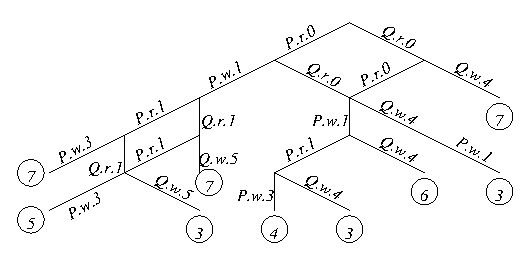
\includegraphics[width=12cm]{interleavings2.eps}\ 
\end{center}
%
The point is that even a very simple program with dependent atomic actions can
become very difficult to understand. 
\end{answer}
 % based on Andrews 2.10; results of particular
                       % interleaving 

% based on Andrews 2.15
\begin{question}
Consider the code below.
%
\begin{scala}
var x = 0; var y = 10

def p = proc{ while(x != y) x = x+1 }

def q = proc{ while(x != y) y = y-1 }

def system = p || q
\end{scala}
%
Will the process \SCALA{system} terminate?  Explain your answer.
\end{question}
%
\begin{answer}
It might or might not terminate.

Consider an execution where we reach a state with \SCALA{x=4} and \SCALA{y=5},
both processes evaluate \SCALA{x!=y} in this state and enter the body of the
loop.  Now suppose each loop body is executed, giving \SCALA{x=5} and
\SCALA{y=4}.  Subsequently we always have \SCALA{x>y}, so neither process
terminates.

Alternatively, again suppose we reach a state with \SCALA{x=4} and
\SCALA{y=5}, both processes evaluate \SCALA{x!=y} in this state and enter the
body of the loop.  Now suppose \SCALA{p} runs, setting \SCALA{x=5}, evaluates
the guard which is now true, and terminates.  However, when \SCALA{q} runs, it
sets \SCALA{y=4}, so never terminates.  Similarly, it is possible
for~\SCALA{q} to terminate, but not~\SCALA{p}.

There are also problems that are caused by the use of caching.  For example,
|p| could reach a state with |x = 6|, while working with |y = 10| in its
cache; and |q| could reach a state with |y = 4|, while working with |x = 0| in
cache.  When they do refresh their caches, they will again run forever.  


It is easy to find executions where both terminate.
\end{answer}
 % based on Andrews 2.15

\begin{question}
Consider a class representing a bounded queue of integers with the following
interface. 
%
\begin{scala}
class Queue{
  def add(value:Int) 
  // Add value to the queue.  
  // Precondition: the queue is not full.

  def remove : Int
  // Remove and return the first element of the queue.
  // Precondition: the queue is not empty.

  def isFull : Bool
  // Test whether the queue is full.

  def isEmpty : Bool
  // Test whether the queue is empty.
}
\end{scala}
%
Assume that each operation is executed atomically.

\begin{enumerate}
\item
Which pairs of operations are independent?

\item
Suppose the queue is shared by two processes:
\begin{itemize}
\item
A \emph{producer}, which (repeatedly) waits until the queue is not full
(tested by repeatedly calling \SCALA{isFull}) and then adds a value to the
queue; 

\item
A \emph{consumer}, which (repeatedly) waits until the queue is not empty
(tested by repeatedly calling \SCALA{isEmpty}) and then removes a value from
the queue.
\end{itemize}
%
Define a \emph{bad} interleaving of the executions of the processes to be
where an operation is called when its precondition does not hold.  Explain why
no bad interleaving can occur.

\item
Now suppose there are two consumers and one producer.  Show that bad
interleavings can occur.
\end{enumerate}


\end{question}

%%%%%

\begin{answer}
\begin{enumerate}
\item
The following pairs of operations are \emph{not} independent: 
\begin{scala}
(ifFull, remove), (isEmpty, add), 
(add, add), (remove, remove), (add, remove)
\end{scala}
The last pair is independent when executed such that the preconditions hold. 

\item
The producer waits until \SCALA{isFull} returns false before attempting
\SCALA{add}.  There may actions by the consumer between those two producer
actions, but they will not make the queue full.  Hence the precondition of
\SCALA{add} holds.

Similarly, actions by the producer between the consumer testing
\SCALA{isEmpty} and calling \SCALA{remove} cannot make the queue empty, so the
precondition of \SCALA{remove} will hold.

\item
Suppose the queue contains one item.  Both consumers test \SCALA{isEmpty},
which returns false.  Now the first consumer calls \SCALA{remove}, which
succeeds, but leaves the queue empty.  Now when the second consumer calls
remove, it fails.
\end{enumerate}
\end{answer}
 %Independent actions of queue -- add, remove, isFull, isEmpty --
              %what can go wrong? Doesn't really work.

\begin{question}
Consider an object representing a bank account, from the following class.
%
\begin{scala}
class Account{
  private var balance = 0

  def credit(value: Int) = atomically{ balance += value }

  def canDebit(value: Int): Boolean = atomically{ balance >= value }

  def debit(value: Int) = atomically{ balance -= value }
}
\end{scala}
%
The ``|atomically|'' pseudocode is intended to indicate that each
procedure is performed atomically (we will see how to do this in a
later chapter).

A process that wants to perform a debit should first of all call
\SCALA{canDebit}, to avoid the account from going overdrawn; for example
%
\begin{scala}[showstringspaces=false]
  if(account.canDebit(value)) account.debit(value)
  else println("Debit not allowed!")
\end{scala}

What can go wrong if two processes execute the above code at the same
time?  Sketch a solution to this problem.
\end{question}

%%%%%

\begin{answer}
Suppose the current balance is 100, and both processes want to debit 100;
clearly only one should succeed.  Both processes could call
\SCALA{canDebit(value)}, getting back the result \SCALA{true}.  They would
then both call \SCALA{debit}, leading to the account balance becoming $-$100.
This is a time-of-check to time-of-use (TOCTTOU) problem: the check that there
is enough money in the account is no longer valid when the debit is
performed. 

The point is that the \SCALA{canDebit} action of one process and the
\SCALA{debit} action of the other are not independent.  This leads to a race
condition.

The obvious way to avoid this problem is to combine the \SCALA{canDebit} and
\SCALA{debit} actions into a single atomic action within the \SCALA{Account}
class.  Something like
%
\begin{scala}
/** Attempt to debit value.  Return true if successful. */
def tryDebit(value: Int): Boolean = atomically{
  if(balance >= value){ balance -= value; true } else false
}
\end{scala}
% 
The calling code (outside the |Account| class) can do the right thing with the
boolean result. 
\end{answer}



\begin{question}
CSO channels are rather like CSP events.  Describe one or two ways in
which they are different.
\end{question}

%%%%%

\begin{answer}
CSP processes are defined in terms of events, and so CSP does not distinguish
between input and output (although there are constructs that behave like input
and output); however, channels in CSO are uni-directional, and so input and
output are distinguished.  This means that if a CSO process is willing to
input from a channel, it should be willing to input an arbitrary value; there
is no equivalent of the CSP selective input, e.g. $in?x:A \then \ldots$.

Also, CSO communications are always synchronisations between exactly two
processes, whereas in CSP any number of processes can synchronise on an
event. 
\end{answer}


\framebox{Problems with Google calendar}

%%%%%

\section{Channels}

\input{mergestreams} % merge two ordered streams

\begin{nontutequestion}
\Programming
\begin{enumerate}
\item
Write a definition for a component
%
\begin{scala}
def zipwith[L,R,O](f:(L, R)=>O)(lin:?[L], rin:?[R], out:![O]) = proc{ ... }
\end{scala}
%
which repeatedly inputs values \SCALA{l} and \SCALA{r} on \SCALA{lin} and
\SCALA{rin}, respectively, and outputs \SCALA{f(l,r)} on \SCALA{out}. 

\item
An \emph{integrator} is a process with signature
%
\begin{scala}
def integrator(in: ?[Int], out: ![Int]) = ...
\end{scala}
that repeatedly inputs on~\SCALA{in}, and outputs on~\SCALA{out} the sums of
the inputs so far.  That is, if it receives the inputs \SCALA{x1, x2, x3,
  ...}, it outputs \SCALA{x1, x1+x2, x1+x2+x3, ...}.  Design and implement an
integrator as a circuit using \SCALA{zipwith} and other common components.
Draw a diagram to explain your design.  Produce a simple test rig to test the
integrator. 
\end{enumerate}
\end{nontutequestion}

%%%%%

\begin{nontuteanswer} 
\begin{scala}
def zipwith[L,R,O](f:(L, R)=>O)(lin:?[L], rin:?[R], out:![O]) = proc{
  var l = null.asInstanceOf[L]; 
  var r = null.asInstanceOf[R];
  repeat { 
    (proc { l = lin? } || proc { r = rin? })(); 
    out!f(l, r) 
  };   
  lin.close; rin.closein; out.closeout
}
\end{scala}
%
In fact, this is defined as \SCALA{ox.cso.Components.zipwith}.

For the integrator, we'll use a circuit like before (where the first component
is a \SCALA{zipwith} using adition.
%
\begin{verbatim}
                in                       out
 [x,y,z,...] >------>|\    mid     /|-------> [x,x+y,x+y+z,...]
                     |+}--------->{ |
                 +-->|/            \|--+
             addl|                     |back
                 +------<prefix 0<-----+
\end{verbatim}
%
\begin{scala}
import ox.CSO._, ox.cso.Components

object Integrator{

  def integrator(in: ?[Int], out: ![Int]) = {
    val mid, back, addl = OneOne[Int]
    (  Components.zipwith ((x:Int, y:Int)=>x+y) (in, addl, mid)
    || Components.tee (mid, List(out, back))
    || Components.prefix(0)(back, addl)
    )
  }

  // Produce stream of nats
  def nats(out: ![Int]) = proc("nats"){
    var n = 0;
    repeat{ out!n; n+=1; sleep(200) }
  }

  // Test rig, using the above
  def TestRig = {
    val in, out = OneOne[Int];
    ( integrator(in, out) || nats(in) || Components.console(out) )
  }

  def main(args : Array[String]) = TestRig()
}
\end{scala}
The test rig provides the integrator with naturals, and we can check that we
get the triangular numbers out.
\end{nontuteanswer}


% \begin{question}
\Programming\
Write a definition for a process
%
\begin{scala}
def Merge(left: ?[Int], right: ?[Int], out: ![Int]) 
= proc ...
\end{scala}
%
that inputs two ascending non-empty streams of integers on \SCALA{left} and
\SCALA{right}, merges them into a single ascending stream, and outputs that on
\SCALA{out}.  The process should hold at most one value at a time from each of
the input streams.  You should think carefully about what to do when one of
the streams is closed. 
% You may not use \SCALA{ox.cso.Components.merge}.
\end{question}
%
\begin{answer}
When one of the input channels is closed, causing the program to break out of
the \SCALA{repeat} loop below, we need to know whether the values of \SCALA{l}
and \SCALA{r} have already been output; we use the flag \SCALA{invalid} for
this.
%
\begin{scala}
import ox.CSO._
import ox.cso.Components._

object MergeStreams{
  // Merge two non-empty ascending streams
  def Merge(left: ?[Int], right: ?[Int], out: ![Int]) 
  = proc("Merge"){
    // Invariant: l is last value read from left; r is 
    // last value read from right; when the repeat loop 
    // exits due to a channel closing, invalid is 0 if the
    // value in l is invalid (has already been output), 
    // and invalid is 1 if the value in r is invalid.
    var l = left?; var r = right?; var invalid = -1;
    repeat{
      if(l<=r){ out!l; invalid=0; l=left? }
      else{ out!r; invalid=1; r=right? }
    }
    println("channel closed")
    if(invalid==1){ out!l; repeat{ out!(left?) } }
    if(invalid==0){ out!r; repeat{ out!(right?) } }
    out.close;
  }

  val random = new scala.util.Random ;

  // Produce an ascending stream of n Ints on out
  def Producer(n:Int, out: ![Int]) = proc("Producer"){
    var current = 0;
    for(i <- 0 until n){ 
      current += random.nextInt(5); 
      println("producing "+current); 
      out!current;
    }
    out.close
  }

  val left = OneOne[Int]; 
  val right = OneOne[Int];
  val out = OneOne[Int];

  def System(n:Int) = (
    Merge(left, right, out) || Producer(n, left) 
    || Producer(n, right) || console(out) 
  )

  def main(args : Array[String]) = 
    System( 
      if(args.length>0)
        Integer.valueOf(args(0)).intValue()
      else 10 
    )();
}
\end{scala}
%
[Students should provide some sensible test results.]
\end{answer}
 % merge two ordered streams, which could be closed

\input{pipeSort} % *** sort list of N numbers using pipe, A7.3

%%%%%

\section{Parallel programming}

\begin{nontutequestion}
In the numerical integration example, we assumed that the number $n$ of
intervals was divisible by the number $ntasks$ of tasks.  How can
we remove this assumption?
\end{nontutequestion}

%%%%%

\begin{nontuteanswer}
The easiest thing to do is to make most tasks of size $\lceil n/ntasks
\rceil$, and to make the last task appropriately smaller.  Making the last
task smaller is likely to make the overall computation finish faster.

It is possible to use a more sophisticated scheme, where all the tasks are of
size $\lceil n/ntasks \rceil$ or $\lfloor n/ntasks \rfloor$, but, frankly,
these don't give any benefits.
\end{nontuteanswer}
 % Remove assumption that \# processors divides \# segments.

\begin{question}
\Programming\ Write a concurrent program to multiply two large $n$ by $n$
matrices~|a| and~|b| together, storing the result in matrix~|c|.  You should
use the bag-of-tasks pattern.  You should consider what a suitable ``task''
should be: remember that making a task too small will mean that workers spend
most of their time waiting to receive the next task.  \textbf{Optional:} carry
out some experiments to assess different sizes of tasks.
% You will probably want to represent each matrix by a two dimensional array.
% Such an array can be initialised in Scala using, e.g.:
% %
% \begin{scala}
% var a = new Array[Array[Int]](N,N);
% \end{scala}
% %
% The element in position $(i,j)$ can be accessed using \SCALA{a(i)(j)}.
\end{question}

%%%%%

\begin{answer}
It makes sense to define a \emph{task} to be the creation of several rows of
the result, say \SCALA{taskSize} rows.  
% The communication overhead is
% $\Theta(n/taskSize)$, so for large arrays, having a task as a single row
% (i.e.\ taking $taskSize=1$) would probably be too small a task (although the
% communication overhead of using a single row would be reasonably small
% compared to the $\Theta(N^3)$ computational cost).  
Taking a task to be a single entry in the result would be too small a task: it
would give a $\Theta(n^2)$ communication overhead.  Using a whole number of
rows (or columns) is easier to program than any other way of splitting up the
problem (e.g.\ into square regions).

There is no need for the workers to return any result to the controller: each
worker can write directly into the result array.  Note that since the tasks
write to disjoint parts of the result array, there are no race conditions. 

Here's my code:
%
\begin{scala}
class Matrix(a: Array[Array[Int]], b: Array[Array[Int]], numWorkers: Int, taskSize: Int){
  private val n = a.size

  /** Array to store the result. */
  private var c = Array.ofDim[Int](n,n)

  /** A task.  The pair (start,end) represents the task of calculating rows [start..end). */
  private type Task = (Int,Int) 

  /** Channel for sending tasks. */
  private val toWorkers = OneMany[Task]

  /** A worker: repeatedly receive tasks, and calculate the relevant rows. */
  private def worker = proc{
    repeat{
      val(start,end) = toWorkers?()
      for(i <- start until end; j <- 0 until n){
	// Calculate value for c(i)(j)
	var sum = 0
	for(k <- 0 until n) sum += a(i)(k)*b(k)(j)
	c(i)(j) = sum
      }
    }
  }

  /** The controller: repeatedly allocate tasks of size taskSize. */
  private def controller = proc{
    var current = 0
    while(current < n){
      toWorkers!(current, current+taskSize min n)
      current += taskSize
    }
    toWorkers.close
  }

  /** calculate the product of a and b. */
  def apply(): Array[Array[Int]] = {
    run(|| (for(w <- 0 until numWorkers) yield worker) || controller)
    c
  }
}
\end{scala}

I ran some informal experiments based around the following function.  The
``warm up'' part is to avoid the effects of JIT compilation.
%
\begin{scala}
  /** Measure times for different task sizes, for matrices of size n and
    * numWorkers worker threads. */
  def timingTest(n: Int, numWorkers: Int) = {
    // # reps; chosen to spend ~3s per task size
    val reps = (300L*Million*numWorkers/(n.toLong*n*n)).toInt
    println("reps = "+reps)
    // Warm up
    for(_ <- 0 until reps){
      val a = randomArray(n); val b = randomArray(n)
      val c = new Matrix(a, b, numWorkers, 2)()
    }
    println("starting")
    for(taskSize <- 1 until 10){
      var elapsed = 0L
      for(_ <- 0 until reps){
        val a = randomArray(n); val b = randomArray(n)
        val start = System.nanoTime
        val c = new Matrix(a, b, numWorkers, taskSize)()
        elapsed += System.nanoTime-start
      }
      println(taskSize+"\t"+elapsed/Million+"ms")
    }
  }
\end{scala}
%
For small values of |n| (around 200) a task size of 2 was often best; with
smaller tasks, the $O(\sm n^2/\sm{taskSize})$ communication overhead meant
that the controller was a bottleneck.  For larger values of |n|, a task size
of~1 was best; each task has $O(\sm n^2)$ computational cost, which is
sufficiently large that the controller is not a bottleneck; and having more
tasks gives better load balancing.  It might be interesting to run experiments
with smaller tasks, say to calculate part of a row of the result.
\end{answer}
 % Matrix multiplication

\begin{nontutequestion}
Suppose you are given two large arrays of |Int|s, |a| and~|b|, neither
of which contains any repetitions.  Describe the design for a
concurrent program to count the number of values that appear in both
arrays.  This problem could be specified (using a couple of functions
from the Scala API) as:
\begin{scala}
  a.count(b.contains(_))
\end{scala}
(You do not need to produce concrete code, unless you want to.)
%%  Briefly explain
%% your design.  
% \textbf{Hint:} use a hash table
% (\url{scala.collection.mutable.HashSet}).  

\end{nontutequestion}

%%%%%

\begin{nontuteanswer}
The easiest way is to split |a| into several segments, one for each worker.
Each worker counts the number of values that appear in both its segment and
in~|b|, and sends the result to a controller.  The controller adds up the
sub-results.  Each worker can calculate its result by putting the elements
of~|b| into a hash table, then counting the number of elements from its
segment that are in the hash table (this avoids quadratic behaviour).  Here's
my code.
%
\begin{scala}
/** Object to count the number of duplicates between a and b, using numWorkers
  * worker threads. */
class CountDups(a: Array[Int], b: Array[Int], numWorkers: Int){
  private val aSize = a.length

  /** Channel for workers to send results to controller. */
  private val toController = ManyOne[Int]

  /** A single worker. */
  private def worker(me: Int) = proc{
    // This worker will deal with a[aStart..aEnd) and all of b
    val aStart = (me*aSize)/numWorkers
    val aEnd = (me+1)*aSize/numWorkers
    // Hash table storing elements of b.
    val bHash = new scala.collection.mutable.HashSet[Int]
    bHash ++= b
    // Iterate through segment of a, counting how many entries are in bHash
    var count = 0
    for(i <- aStart until aEnd; if bHash.contains(a(i))) count += 1 
    // Send result to controller
    toController!count
  }

  /** Variable that ends up holding the result.  While the system is running,
    * only the controller writes to this, and no other thread reads it, so
    * there are no races. */
  private var result = 0

  /** The controller. */
  private def controller = proc{
    for(i <- 0 until numWorkers) result += toController?()
  }

  /** Find the number of duplicates. */
  def apply(): Int = {
    result = 0
    // Run the system
    run(|| (for(i <- 0 until numWorkers) yield worker(i)) || controller)
    result
  }	
}
\end{scala}

An alternative would be to use the bag-of-tasks pattern, where each task
corresponds to a segment of~|a|; note that each worker can re-use its hash
table for multiple tasks. 

There seems no point in splitting \emph{both} |a| and~|b| into multiple
segments, as this wouldn't allow the hash table to be re-used.  

In fact, it is probably sound for the workers to share a single hash table
|bHash| that stores the values from~|b|, as long as all the elements of~|b| are
added to |bHash| before any worker starts.  This assumes that the |contains|
operation for the hash table is thread-safe (i.e.~two threads can safely perform
|contains| concurrently); this will be the case if |contains| performs no
write of a variable (which will often be the case).  It is tempting to arrange
for the workers to share the work of adding the elements of |b| to |bHash|.
However, the |add| operation on the hash table almost certainly isn't
thread-safe; we will see in later chapters how to design a concurrent
datatype, like a hash table, that is thread-safe. 

Testing can be performed by generating random arrays with no repetitions,
running the concurrent algorithm, and then comparing with the result specifed
in the question; this can be repeated many times.
\end{nontuteanswer}


%%% Old version, which doesn't make a lot of sense.

% The obvious approach is to split \SCALA{a} into \SCALA{aSegs} segments, and
% \SCALA{b} into \SCALA{bSegs} segments, and to give a segment of \SCALA{a}
% and a segment of \SCALA{b} to each worker (possibly several pairs of segments,
% but see below).  The worker can count the number of common values in these
% segments by putting the elements of the segment of \SCALA{b}, say, into a hash
% table, and then testing whether each element of the segment of \SCALA{a} is in
% that hash table.  The counts from each worker can be passed to a
% controller,that adds them up. 

% Should we use the bag of tasks pattern, or should each worker deal with a
% single segment of each array?
% A bit of thought shows that taking \SCALA{aSegs*bSegs} greater than the number
% of processes leads to duplicated work: splitting a segment of~\SCALA{a} into
% multiple segments means that the hash table for the segment of~\SCALA{b} has
% to be created extra times; and splitting a segment of~\SCALA{b} into multiple
% segments means that each element of~\SCALA{a} has to be dealt with extra
% times.  We therefore avoid the bag of tasks pattern, and allocate a single
% segment of each array to each worker.  

% Code is not compulsory, but I'll include mine below, anyway.  My experiments
% suggest that this is fastest (on an 8 processor machine) when we take
% \SCALA{aSegs = 1} and \SCALA{bSegs = 8}.  This is an artefact of the relative
% speeds of different operations, and I don't think could have been anticipated
% in advance. 


%% We split \SCALA{a} into \SCALA{aSegs} segments, and \SCALA{b} into
%% \SCALA{bSegs} segments.  Each of the \SCALA{numWorkers = aSegs*bSegs} workers
%% wil work on a segment of \SCALA{a} and a segment of~\SCALA{b}, and count the
%% number of values that appear in both segments, and send the result to the
%% controller.  The elements of the \SCALA{b} segment are put into a hash table
%% to allow fast checking of membership.
%
% \begin{scala}
% // Given arrays a, b, with no repetitions, count the 
% // number of distinct elements in both a and b.

% import ox.CSO._;

% object CountDups{
%   val N = 500000; // size of arrays
%   val a = new Array[Int](N);
%   val b = new Array[Int](N);

%   // Each worker will work on a segment of a and 
%   // a segment of b
%   val aSegs = 1; // number of segments of a
%   val aSegSize = N/aSegs
%   val bSegs = 8; // number of segments of b
%   val bSegSize = N/bSegs
%   val numWorkers = aSegs*bSegs; 

%   // A single worker
%   def Worker(me: Int, toController: ![Int]) = proc{
%     // This worker will deal with a[aStart..aEnd) 
%     // and b[bStart..bEnd) 
%     def aStart = (me/bSegs) * aSegSize;
%     def aEnd = (me/bSegs + 1) * aSegSize;
%     def bStart = (me%bSegs) * bSegSize;
%     def bEnd = (me%bSegs + 1) * bSegSize;

%     // Put all b elements in hash table
%     // val bHash = new java.util.HashSet[Int](bSegSize*2);
%     // for(i <- bStart until bEnd) bHash.add(b(i));
%     val bHash = new scala.collection.mutable.HashSet[Int];
%     for(i <- bStart until bEnd) bHash += b(i);

%     // Now iterate through segment of a, counting how 
%     // many entries are in bHash
%     var count = 0;
%     for(i <- aStart until aEnd)
%       if(bHash.contains(a(i))) count+=1;

%     // Send result to controller
%     toController!count;
%   }

%   // The controller
%   def Controller(toController: ?[Int]){
%     var count = 0;
%     for(i <- 0 until numWorkers) count += (toController?);
%     println(count);
%   }

%   // Initialise arrays
%   def Init{
%     // We set a(i)=i, b(i)=2*i;
%     for(i <- 0 until N){ a(i)=i; b(i)=2*i; }
%   }

%   // Construct system
%   val toController = ManyOne[Int];
%   def Workers =
%     || ( for(i <- 0 until numWorkers) yield 
%            Worker(i, toController) )
%   def System = Controller(toController) || Workers

%   def main(args:Array[String]) = {
%     Init; 
%     val t0 = java.lang.System.currentTimeMillis();
%     System();
%     println("Time taken: "+
%       (java.lang.System.currentTimeMillis()-t0)/1000.0);
%   }
% }
% \end{scala}

% Curiously, the Scala hashtable seems considerably faster than the Java one. 
% \end{nontuteanswer}

% Given two arrays a and b, without repetitions, count the number of distinct
% elements that appear in both a and b. 

% \begin{question}
\Programming\
Suppose you are given two arrays, as follows:
%
\begin{scala}
  val N = ...;
  val a = new Array[Int](N);
  val b = new Array[Int](N);
\end{scala}
%
Neither array contains any repetitions.  Write a concurrent program to count
the number of distinct values that appear in both arrays.  Briefly explain
your design.  \textbf{Hint:} use a hash table
(\url{scala.collection.mutable.HashSet}).   
\end{question}

%%%%%

\begin{answer}
We split \SCALA{a} into \SCALA{aSegs} segments, and \SCALA{b} into
\SCALA{bSegs} segments.  Each of the \SCALA{numWorkers = aSegs*bSegs} workers
wil work on a segment of \SCALA{a} and a segment of~\SCALA{b}, and count the
number of values that appear in both segments, and send the result to the
controller.  The elements of the \SCALA{b} segment are put into a hash table
to allow fast checking of membership.
%
\begin{scala}
// Given arrays a, b, with no repetitions, count the 
// number of distinct elements in both a and b.

import ox.CSO._;

object CountDups{
  val N = 500000; // size of arrays
  val a = new Array[Int](N);
  val b = new Array[Int](N);

  // Each worker will work on a segment of a and 
  // a segment of b
  val aSegs = 1; // number of segments of a
  val aSegSize = N/aSegs
  val bSegs = 8; // number of segments of b
  val bSegSize = N/bSegs
  val numWorkers = aSegs*bSegs; 

  // A single worker
  def Worker(me: Int, toController: ![Int]) = proc{
    // This worker will deal with a[aStart..aEnd) 
    // and b[bStart..bEnd) 
    def aStart = (me/bSegs) * aSegSize;
    def aEnd = (me/bSegs + 1) * aSegSize;
    def bStart = (me%bSegs) * bSegSize;
    def bEnd = (me%bSegs + 1) * bSegSize;

    // Put all b elements in hash table
    // val bHash = new java.util.HashSet[Int](bSegSize*2);
    // for(i <- bStart until bEnd) bHash.add(b(i));
    val bHash = new scala.collection.mutable.HashSet[Int];
    for(i <- bStart until bEnd) bHash += b(i);

    // Now iterate through segment of a, counting how 
    // many entries are in bHash
    var count = 0;
    for(i <- aStart until aEnd)
      if(bHash.contains(a(i))) count+=1;

    // Send result to controller
    toController!count;
  }

  // The controller
  def Controller(toController: ?[Int]){
    var count = 0;
    for(i <- 0 until numWorkers) count += (toController?);
    println(count);
  }

  // Initialise arrays
  def Init{
    // We set a(i)=i, b(i)=2*i;
    for(i <- 0 until N){ a(i)=i; b(i)=2*i; }
  }

  // Construct system
  val toController = ManyOne[Int];
  def Workers =
    || ( for(i <- 0 until numWorkers) yield 
           Worker(i, toController) )
  def System = Controller(toController) || Workers

  def main(args:Array[String]) = {
    Init; 
    val t0 = java.lang.System.currentTimeMillis();
    System();
    println("Time taken: "+
      (java.lang.System.currentTimeMillis()-t0)/1000.0);
  }
}
\end{scala}

My experiments suggest that this is fastest (on an 8 processor machine) when
we take \SCALA{aSegs = 1} and \SCALA{bSegs = 8}.

Curiously, the Scala hashtable seems considerably faster than the Java one. 
\end{answer}
 % Same but give full code

\framebox{Travelling salesman?}  Andrews 9.7

\begin{nontutequestion}
(Optional.)
\begin{enumerate}
\item
Suppose $x$ and $y$ are random numbers, chosen with a uniform distribution on
$[0,1)$.  Show that $Prob(x^2+y^2<1) = \pi/4$.  Hint: use a geometric
  argument.

\item
\Programming\ 
Use this idea to write a concurrent program to estimate the value of $\pi$.

\item
(For those who have taken a course on probability:) Estimate the
  standard deviation of the results given by your program.
\end{enumerate}
\end{nontutequestion}

%%%%%

\begin{nontuteanswer}
For part (a): consider a quarter circle, with centre $(0,0)$, inscribed in the
quadrant $0 \le x,y < 1$.  Then
\begin{eqnarray*}
Prob(x^2+y^2<1) & = & Prob(\mbox{$(x,y)$ is in the quarter circle}) \\
 & = & \mbox{area of quarter circle}/\mbox{area of quadrant} \\
 & = & \pi/4.
\end{eqnarray*}

The program below uses the bag of tasks pattern.  Each task is to generate
\SCALA{taskSize} pairs $(x,y)$ and to count how many satisfy $x^2+y^2<1$.  The
controller compiles the results.
%
\begin{scala}
// Estimate pi, using the fact that if x, y are random 
// numbers in [0,1), then P(x^2+y^2)<1 = pi/4.

import ox.CSO._

object pi{
  val taskSize = 20000;
  val numTasks = 50;
  val numWorkers = 8;

  // val random = new scala.util.Random;

  // The worker receives a signal on toWorkers, generate
  // taskSize random pairs (x,y), and tell controller 
  // (on toController) how many had x^2+y^2 < 1.
  def Worker(toWorkers: ?[Unit], toController: ![Int]) 
  = proc{
    val random = new scala.util.Random;
    repeat{
      toWorkers?;
      var count=0;
      for(i <- 0 until taskSize){
	val x = random.nextDouble; 
        val y = random.nextDouble;
	if(x*x+y*y<1.0) count += 1;
      }
      toController!count;
    }
  }

  def Controller(toWorkers: ![Unit], toController: ?[Int]) 
  = proc{
    // Process to distribute numTasks tasks
    def Sender = proc{
      for(i <- 0 until numTasks) toWorkers!();
      toWorkers.close
    }

    // Process to receive counts and calculate result
    def Receiver = proc{
      var count:Int = 0;
      for(i <- 0 until numTasks) count += (toController?) ;
      println( 
        (4.0*(count:Double)/(taskSize*numTasks)).toString
      );
    }

    (Sender || Receiver)();
  }

  // Construct system
  val toWorkers = OneMany[Unit];
  val toController = ManyOne[Int];
  
  def Workers = 
    || ( for(i <- 0 until numWorkers) yield
           Worker(toWorkers, toController) );

  def System = 
    Controller(toWorkers, toController) || Workers

  def main(args:Array[String]) = {
    val t0 = java.lang.System.currentTimeMillis();
    System();
    println("Time taken: "+
      (java.lang.System.currentTimeMillis()-t0)/1000.0);
  }
}
\end{scala}

Each worker can be given their own random number generator, or they can share
a single one.  In my tests, the latter is about 20 times slower, which is quite
surprising.  I suspect the reason it is more than \SCALA{numWorkers} times
slower is that the state of the random number generator has to be copied to
the appropriate cache for each random number.

If we let $n$ be the number of samples, then the number of samples that
satisfy the property $x^2+y^2<1$ has binomial distribution $Binom(n,\pi/4)$,
which has variance $n.\pi/4.(1-\pi/4)$, standard deviation
$\sqrt(n.\pi/4.(1-\pi/4))$, and so a standard deviation on the final result of
$4.\sqrt(\pi/4.(1-\pi/4)) / \sqrt n \approx 1.64 / \sqrt n$.  For $n = 10^6$, as
above, this is about $0.00164$.  This is consistent with the experimental
observation that the program is normally accurate to about two decimal places.
\end{nontuteanswer}
 % *** Estimating pi: pick random numbers x, y in [0,1);  prob$(x^2+y^2)<1 = \pi/4$. 

%%%%%


\section{Alternation}

\begin{question}
% \Programming\
Write a definition for a process
%
\begin{scala}
def Interleave(left: ?[Int], right: ?[Int], out: ![Int]) = proc ...
\end{scala}
that inputs two streams of integers on \SCALA{left} and \SCALA{right},
interleaves them into a single stream (in some order), and outputs that on
\SCALA{out}.  You should think carefully about what to do when one of the
streams is closed.  You may not use \SCALA{ox.cso.Components.merge}.

Discuss whether your implementation is \emph{fair} to the two input streams. 
\end{question}

%%%%%

\begin{answer}
\Small
\begin{scala}
  def Interleave(left: ?[Int], right: ?[Int], out: ![Int]) 
  = proc("Interleave"){
    serve(
      left --> { out!(left?); }
      | right --> { out!(right?) }
    )
    repeat{ out!(left?); }
    repeat{ out!(right?); }
    left.close; right.close; out.close;
  }
\end{scala}
%% \begin{scala}
%% import ox.CSO._
%% import ox.cso.Components._

%% object Interleave{

%%   // Merge two streams
%%   def Interleave(left: ?[Int], right: ?[Int], out: ![Int]) 
%%   = proc("Interleave"){
%%     serve(
%%       left --> { out!(left?); }
%%       | right --> { out!(right?) }
%%     )
%%     repeat{ out!(left?); }
%%     repeat{ out!(right?); }
%%     out.close;
%%   }

%%   val random = new scala.util.Random ;

%%   // Produce an ascending stream of n Ints on out
%%   def Producer(me: Int, n:Int, out: ![Int]) 
%%   = proc("Producer"){
%%     for(i <- 0 until n){ 
%%       val current=random.nextInt(10); 
%%       println(me+" producing "+current); out!current;
%%       sleep(random.nextInt(50));
%%     }
%%     out.close
%%   }

%%   val left = OneOne[Int]; 
%%   val right = OneOne[Int];
%%   val out = OneOne[Int];

%%   def System(n:Int) = (
%%     Interleave(left, right, out) || 
%%     Producer(1, n, left) || Producer(2, n, right)
%%     || console(out) 
%%   )

%%   def main(args : Array[String]) = 
%%     System( 
%%       if(args.length>0){
%%         Integer.valueOf(args(0)).intValue()
%%       } else 10 
%%     )();
%% }
%% \end{scala}

This is fair in the sense that if both channels are ready to communicate, it
will alternate between them, because that's the sense in which \SCALA{serve}
is fair. 
\end{answer}
 

\begin{nontutequestion}
Design a \emph{change machine} process with signature:
%
\begin{scala}
def ChangeMachine(inPound: ?[Unit], out5p: ![Unit], out10p: ![Unit], out20p: ![Unit])
\end{scala}
%
where communications on the channels correspond to the insertion of \pounds 1,
and the output of a 5p, 10p or 20p piece, respectively.  It should be willing
to accept \SCALA{inPound} whenever it had a zero balance.  It should offer
the environment the choice between how it wants the change, subject to the
condition that it should not output coins of more value than it has received. 
\end{nontutequestion}

%%%%%

\begin{nontuteanswer}
\Small
\begin{scala}  
def ChangeMachine(inPound: ?[Unit], out5p: ![Unit], out10p: ![Unit], out20p: ![Unit]) = proc{
  var credit = 0 // credit in pence
  serve(
    (credit == 0 && inPound) =?=> { () => credit += 100 }
    | (credit >= 5 && out5p) =!=> { credit -= 5; () }
    | (credit >= 10 && out10p) =!=> { credit -= 10; () }
    | (credit >= 20 && out20p) =!=> { credit -= 20; () }
  )
}
\end{scala}
\end{nontuteanswer}


\begin{question}
The CSO construct \SCALA{alt} is rather like the external choice operator
$\extchoice$.  Describe a couple of ways in which they are different.
\end{question}

%%%%%

\begin{answer}
\begin{itemize}
\item
\SCALA{alt} operates over channels, whereas $\extchoice$ operates over
arbitrary processes.  For example, in CSP you can have a process such as
\[
(P \parallel Q) \extchoice (R \intchoice S)
\]
but you can't achieve a similar effect using \SCALA{alt}. 

\item
In CSO, if the outport of a channel is involved in an \SCALA{alt}, the inport
may not simultaneously be involved in an(other) \SCALA{alt}.  But in CSP it's
fine to have a process such as
\[
(c!x \then \ldots \extchoice \ldots) \parallel (c?x \then \ldots \extchoice
\ldots). 
\]
\end{itemize}
\end{answer}


\begin{nontutequestion}
Recall the following restriction on the use of \SCALA{alt}:
%
\begin{quote}
If the output port of a channel participates in an \SCALA{alt} then its input
end must not simultaneously participate in an(other) \SCALA{alt}.
\end{quote}
%
Suggest a reason for this restriction.
\end{nontutequestion}

%%%%%

\begin{nontuteanswer}
The restriction makes implementation of \SCALA{alt} much easier.  Consider a
program such as \SCALA{P || Q} where:
%
\begin{scala}
def P = proc{ alt( c -!-> ... | a -?-> ...) }
def Q = proc{ alt( c -?-> ... | b -?-> ...) }
\end{scala}
%
The two \SCALA{alt}s are executed by different threads.  There is a danger of
the \SCALA{alt} in \SCALA{P} selecting channel~\SCALA{c} at the same time that
the \SCALA{alt} in \SCALA{Q} selects channel~\SCALA{b}, for example; the two
threads would then evolve in ways inconsistent with the intended semantics.    

Solving these problems would require some non-trivial synchronisation between
the two threads.

This problem potentially becomes harder when we have more than two processes.

Very similar examples can be used to show why the input port of a OneMany
channel may not simultaneously participate in more than one \SCALA{alt}. 
\end{nontuteanswer}

%% Consider a ring of processes:
%% %
%% \begin{scala}
%% || ( for(i <- 0 until N) yield P(i) )
%% \end{scala}
%% %
%% where
%% %
%% \begin{scala}
%% def P(me) = proc{ alt( c((me+1)\%N) -!-> ... | c(me) -?-> ...) }
%% \end{scala}


\begin{question}
% \Programming\
Implement an unbounded buffer as a process:
%
\begin{scala}
def buff[T](in: ?[T], out: ![T]) = proc{ ... }
\end{scala}
%
The process should always be willing to input on \SCALA{in}; it should output
data on \SCALA{out} in the order in which they were received, and should be
willing to output whenever it has input data that have not yet been output. 

{\bf Hint:} you might want to use an instance of a
\SCALA{scala.collection.mutable.Queue} to store the current values held in the
buffer.
\end{question}

%%%%%

\begin{answer}
\Small
\begin{scala}
  def buff[T](in: ?[T], out: ![T]) = proc{
    var queue = new scala.collection.mutable.Queue[T]

    serve(
      in =?=> { x => queue.enqueue(x) }
      | (queue.nonEmpty && out) =!=> { queue.dequeue }
    )
  }
\end{scala}
%
We will discuss testing of datatypes like this later in the course.  For the
moment, I would expect to see some testing involving some threads passing in
pre-defined sequences of values, and other threads taking the outputs and
writing them into global variables, and then checking that the outputs are a
permutation of the inputs. 
%
%% The testing harness is designed to allow data to accumulate in the buffer ---
%% and that's what the test results show.
\end{answer}
%% \begin{answer}
%% \begin{scala}
%% import ox.CSO._

%% object UnboundedBuff{
%%   // Unbounded buffer
%%   def Buff[T](in: ?[T], out: ![T]) = proc{
%%     var queue = new scala.collection.mutable.Queue[T];

%%     serve(
%%       in -?-> { queue.enqueue(in?); }
%%       | (!queue.isEmpty &&& out) -!-> { out!(queue.dequeue); }
%%     )
%%   }

%%   // Produce stream of nats
%%   def Nats(out: ![Int]) = proc("nats"){
%%     var n = 0;
%%     repeat{ out!n; println("Sent "+n); n+=1; sleep(400) }
%%   }

%%   // Consume and print numbers at random intervals
%%   def Console(in: ?[Int]) = proc{
%%     val random = new scala.util.Random;
%%     repeat{ sleep(random.nextInt(1000)); println(in?); }
%%   }

%%   val in, out = OneOne[Int];
%%   def System = Nats(in) || Buff(in, out) || Console(out)

%%   def main(args : Array[String]) = System()
%% }
%% \end{scala}
%% %
%% The testing harness is designed to allow data to accumulate in the buffer ---
%% and that's what the test results show.
%% \end{answer}


\begin{nontutequestion}
\Programming\
Recall the integrator network from the previous sheet.  Adapt the network so
that it has an additional input channel 
\SCALA{reset : ?[Unit]}, such that when it receives a signal on
\SCALA{reset}, the current sum gets reset to 0.  Explain your design.  {\bf
  Hint:} you only need to change one component of the network.
\end{nontutequestion}

%%%%%

\begin{nontuteanswer}
\Small
We replace the \SCALA{prefix(0)} component with a new component
\SCALA{Control} which handles the resets:
%
\begin{verbatim}
                in                       out
 [x,y,z,...] >------>|\    mid     /|-------> [x,x+y,x+y+z,...]
                     |+}--------->{ |
                 +-->|/            \|--+
             addl|                     |back
                 +------<Control<------+
                           /|\
                            |
                          reset
\end{verbatim}
%
It's also possible to put the resetting component elsewhere in the network.

Note that \SCALA{Control} needs to absorb the sum currently circulating before
(or after) injecting a fresh value~$0$.  It makes sense to give \SCALA{reset}
priority over values currently circulating.
%
\begin{scala}
import ox.CSO._, ox.cso.Components

object ResettableIntegrator{

  def Control(in: ?[Int], out: ![Int], reset: ?[Unit]) 
  = proc{
    out!0;
    priserve(
      reset --> { 
        reset?; println("Resetting"); in?; out!0 
      }
      | in --> { out!(in?) }
    )
  }  

  def integrator(in: ?[Int], out: ![Int], reset: ?[Unit])
  = {
    val mid, back, addl = OneOne[Int]
    (Components.zipwith((x:Int, y:Int)=>x+y)(in, addl, mid)
    || Components.tee (mid, List(out, back))
    || Control(back, addl, reset)
    )
  }

  // Produce stream of nats
  def Nats(out: ![Int]) = proc("nats"){
    var n = 0;
    repeat{ out!n; n+=1; sleep(200) }
  }

  // Randomly reset
  def Resetter(reset: ![Unit]) = proc{
    val random = new scala.util.Random;
    repeat{ sleep(random.nextInt(1000)); reset!(); }
  }  

  // Test rig, using the above
  def TestRig = {
    val in, out = OneOne[Int]; val reset = OneOne[Unit];
    ( integrator(in, out, reset) || 
     Nats(in) || Resetter(reset) || 
     Components.console(out) )
  }

  def main(args : Array[String]) = TestRig()
}
\end{scala}

\end{nontuteanswer}


\framebox{Traffic lights?}


%%%%%

\section{Clients and Servers} % A7.6: Readers \& Writers 

\begin{nontutequestion}
\Programming\ 
The \emph{readers and writers problem} is a classic synchronisation problem.
Consider a collection of processes, each of which want to access a database
concurrently, some for reading and some for writing.  It is allowable for
several readers to be accessing the database simultaneously, since their
transactions will be independent.  However, it is not allowable for two
writers to have simultaneous access, nor for a reader and writer to have
simultaneous access.

Implement a solution to the readers and writers problem using a server
process: each reader and writer should communicate with the server when
entering or leaving.

Is a reader or writer who is trying to gain entry to the database guaranteed
to succeed, or could it be locked out forever?  If the latter, how could this
be avoided? 
\end{nontutequestion}

%%%%%

\begin{nontuteanswer}
\Small
The server needs to keep track of the numbers of readers and writers currently
accessing the database, and maintain the invariant
\[
(readers=0 \land writers \le 1) \lor writers=0
\]

Avoiding starvation is tricky, since, say readers may always gain access,
locking the writers out for ever.  Below, priority is given to processes
wishing to leave, and when $readers=0 \land writers=0$, it alternates between
giving priority to a reader or a writer (according to the flag
\SCALA{writerPri}).    
%
\begin{scala}[showstringspaces=false]
// The readers and writers problem
import ox.CSO._

object ReadersWriters{
  val random = new scala.util.Random;

  // A reader, which just repeatedly enters and leaves
  def Reader(me: Int, enter: ![Int], leave: ![Int]) = proc{
    repeat{
      sleep(random.nextInt(2000)); enter!me;
      sleep(random.nextInt(1000)); leave!me
    }
  }

  // A reader, which does likewise
  def Writer(me: Int, enter: ![Int], leave: ![Int])= proc{
    repeat{
      sleep(random.nextInt(2000)); enter!me;
      sleep(random.nextInt(1000)); leave!me
    }
  }

  // A server which controls the entering and leaving, 
  // maintaining the invariant: (readers==0 && writers<=1) || writers==0
  // Priority is always given to leaving.  When readers==0 and writers==0, 
  // priority is given to a writer to enter next iff writerPri
  def Server(readerEnter: ?[Int], readerLeave: ?[Int],
	     writerEnter: ?[Int], writerLeave: ?[Int])
  = proc{
    var readers = 0; var writers = 0;
    def Report = { println("readers="+readers+"; writers="+writers); }
    var writerPri = true; // Does writer get priority?

    priserve(
      (readers>0 &&& readerLeave) --> {
	val id = readerLeave?; readers-=1; println("Reader "+id+" leaves"); Report
      }
      | 
      (writers>0 &&& writerLeave) --> {
	val id = writerLeave?; writers-=1; println("Writer "+id+" leaves"); Report
      }
      | 
      (writerPri && readers==0 && writers==0 &&& writerEnter) --> {
	val id = writerEnter?; writers+=1; writerPri=false;
	println("Writer "+id+" enters"); Report
      }
      |
      (writers==0 &&& readerEnter) --> {
	val id = readerEnter?; readers+=1; writerPri=true;
	println("Reader "+id+" enters"); Report
      }
      | 
      (!writerPri && readers==0 && writers==0 &&& writerEnter) --> {
	val id = writerEnter?; writers+=1; writerPri=false;
	println("Writer "+id+" enters"); Report
      }
    )
  }

  // Number of readers and writers:
  val readers = 5; val writers = 5

  // Declare the channels
  val readerEnter, readerLeave, writerEnter, writerLeave = ManyOne[Int];  

  def Readers = 
    || ( for(i <- 0 until readers) yield Reader(i, readerEnter, readerLeave) )
  def Writers =
    || ( for(i <- 0 until readers) yield Writer(i, writerEnter, writerLeave) )
  def System = 
    Readers || Writers || Server(readerEnter,readerLeave,writerEnter,writerLeave)

  def main(args : Array[String]) = { System() }
}
\end{scala}

This does not guarantee starvation freedom, since the readers may try to enter
sufficiently often that $readers$ never reaches zero, so no writer can gain
entry.  This can be avoided by having writers register their interest (by
another communication, that the server always accepts), and then not allowing
any more \SCALA{readerEnter} events before a \SCALA{writerEnter} event.
\end{nontuteanswer}



\input{menWomenServer}

\framebox{Elevator algorithm?}

\framebox{Several-caster} 2008 exam, Q2

\framebox{Multi-casting connections} 2008 exam, Q3

\framebox{Consider} a set of processes where each process is identified by
a unique integer. Each process has a constrained region, which can be entered
only if the sum of all integers associated with processes already executing in
their constrained regions is divisible by three.  Implement this in a
client-server pattern.  Is it possible for a process to be locked out?

\begin{question}
\Programming\ (Based on Andrews, Exercise 7.8.)  
%
A savings account is shared by several people.  Each person may deposit or
withdraw funds from the account, but the balance may never become negative.  

Develop a server to model this problem.  Withdrawal operations must be queued
until there are sufficient funds available.  (You might like to use a
\url{scala.collection.mutable.Queue} to hold such queued withdrawals.)
\end{question}

%%%%%

\begin{answer}
\begin{scala}
import ox.CSO._

object SavingsAccount{
  type ClientId = Int;
 
  abstract class Request;
  case class Deposit(amount:Int, c:ClientId) extends Request; 
  case class WithDrawal(amount:Int, c:ClientId) extends Request;

  abstract class Response;
  case class Ok() extends Response; 
 
  // The server
  def Server(req: ?[Request], resp: Seq[![Response]]) = proc{
    var balance = 0; // current balance
    // queue of withdrawal requests not yet serviced
    val queue = new scala.collection.mutable.Queue[Request] 

    repeat{
      val request = req?;
      request match{
	case Deposit(amount, c) => {
	  balance += amount;
	  resp(c) ! new Ok();
	  println("Deposit of "+amount+"; balance now "+balance);
	  // See if any queued withdrawals can be serviced
	  var done = false;
	  while(! queue.isEmpty && !done){
	    queue.front match{
	      case WithDrawal(amount1, c1) => {
		if(amount1<=balance){
		  queue.dequeue; balance -= amount1; 
                  resp(c1) ! new Ok();
		  println("Withdrawal of "+amount1+ 
                    " dequeued; balance now "+balance);
		} 
		else done = true;
	      }
	    }
	  }
	}
	case WithDrawal(amount, c) => {
	  if(amount<=balance){
	    balance -= amount; resp(c) ! new Ok();
	    println("Withdrawal of "+amount+
                    "; balance now "+balance);
	  }
	  else{
	    queue += request;
	    println("Withdrawal of "+amount+" queued");
	  }
	}
      }
    }
  }

  val random = new scala.util.Random;

  def Client(me: ClientId, req: ![Request], resp: ?[Response]) 
  = proc{
    repeat{
      if(random.nextInt(2)==0){	// Make deposit
	req ! new Deposit(random.nextInt(10), me);
	resp?; ()
      }
      else{ // Make withdrawal
	req ! new WithDrawal(random.nextInt(10), me);
	resp?; ()
      }
      sleep(random.nextInt(2000))
    }
  }

  val numClients = 5;

  val req = ManyOne[Request];
  val resp = OneOne[Response](numClients);
	  
  def Clients =
    || (for (c <- 0 until numClients) yield
          Client(c, req, resp(c)) )

  def System = Clients || Server(req, resp)

  def main(args:Array[String]) = System();
}
\end{scala}

There are a number of possible variations.  The above implementation services
a new withdrawal request, even if there are others queued; alternatively it
could be added to the back of the queue.  The above implementation only tries
to service queued withdrawal requests in queue order, until one is found that
is for too much; there might be withdrawal requests for smaller amounts
further down the queue that could be serviced immediately.

The system can deadlock if all clients try to make withdrawals for which
insufficient funds are available.  This seems unavoidable.
\end{answer}
	  
 % A7.8 Savings account problem

\begin{question}
\Programming\ (Based on Andrews, Exercise 7.11.)
%
Cars coming from the north and the south arrive at a one-lane bridge.  Cars
heading in the same direction can cross the bridge at the same time, but cars
heading in the opposite direction cannot.

Develop a server process to manage use of the bridge.  Assume that cars are
client processes.  Describe the protocol between the cars and the server.
\end{question}

%%%%%

\begin{answer}
The protocol is that cars send a Arrive message when they arrive, wait for
an acknowledgement (a Unit), cross the bridge, then send a Leave message.
The server allows cars to proceed if there is no car crossing or waiting to
cross in the opposite direction; otherwise the car queues.
%
\begin{scala}
import ox.CSO._;

object OneLaneBridge{
  type ClientId = Int;
 
  abstract class Request;
  case class Arrive(fromN:Boolean, c:ClientId) extends Request;
  case class Leave(c:ClientId) extends Request;

  // The server
  def Server(req: ?[Request], resp: Seq[![Unit]]) = proc{
    var currentN = true; // is current priority from north?    
    // Queue of cars queuing in the opposite direction  
    var queue = new scala.collection.mutable.Queue[ClientId] 
    // Queues going in the current direction, now queueing
    var nextQueue = new scala.collection.mutable.Queue[ClientId] 
    var count = 0; // number of cars currently crossing

    // Convert direction to string
    def showDir(isN:Boolean) = if(isN) "North" else "South";

    repeat{
      req? match{
	case Arrive(fromN, c) => {
	  if(fromN==currentN){ // Car going in current direction
	    if(queue.isEmpty){ // Allow to proceed
	      resp(c)!(); count += 1;
	      println("Car "+c+" arrives from "+
		      showDir(fromN)+" and proceeds")
	    } else { // Must wait
	      nextQueue += c;
	      println("Car "+c+" arrives from "+
		      showDir(fromN)+" and queues")
	    }
	  }
	  else if(count==0){ 
            // Reverse direction, allow to proceed
	    currentN = fromN; resp(c)!(); count = 1;
	    println("Car "+c+" arrives from "+
		    showDir(fromN)+" and proceeds")
	  } else { // Add to queue
	    queue += c;
	    println("Car "+c+" arrives from "+
		    showDir(fromN)+" and queues")
	  }
	}
	case Leave(c) => { // Detect a car has left
	  count -= 1;
	  println("Car "+c+" leaves");
	  if(count==0 && !queue.isEmpty){ // Reverse direction
	    currentN = !currentN;
	    // Set the queue going
	    while(!queue.isEmpty){ 
	      val c = queue.dequeue; resp(c)!(); count += 1;
	      println("Car "+c+" dequeued, and continues "+
		      showDir(currentN))
	    }
	    // Swap the queues
	    val temp = queue; 
            queue = nextQueue; nextQueue = queue;
	  }
	}
      }
    }
  }

  val random = new scala.util.Random;

  // A car
  def Car(me: Int, req: ![Request], resp: ?[Unit]) = proc{
    repeat{
      sleep(random.nextInt(8000));
      // Arrive from random direction
      req!Arrive(random.nextInt(2)==0, me); 
      resp?; // Wait for permission 
      sleep(random.nextInt(2000)); // Cross the bridge
      req!Leave(me); // And away
    }
  }

  // Put system together
  val numCars = 5;
  val req = ManyOne[Request];
  val resp = OneOne[Unit](numCars);

  def Cars = 
    || ( for(i <- 0 until numCars) yield Car(i, req, resp(i)) )

  def System = Server(req, resp) || Cars

  def main(args:Array[String]) = System();
}
\end{scala}
\end{answer}
 % ***? A7.11 One-lane bridge

%%%%%

\section{Interacting Peers}

% Loosely based on A7.9
\begin{question}
\Programming\ Consider a setting with two kinds of processes, which we will
call Male and Female; suppose we have $N$ Males and $N$ Females.  The aim is
to pair the processes off for some purpose, so each Male is paired with a
Female, and vice versa.  Each process should end up in possession of its
partner's identity.  Design and implement a protocol to achieve this.  The
protocol should be such that the pairings are decided nondeterministically (so
it's not acceptable for the protocol to simply pair each Male off with the
Female with the same index, for example).  The protocol should not use any
process other than the Males and Females.  Note: you need to be careful to
follow the restrictions on the use of \SCALA{alt}s.
\end{question}

%%%%%

\begin{answer}
We will arrange (arbitrarily) for the Female to send a ``proposition'' to a
Male, and she is willing for any Male to receive this; each Male will accept a
single proposition, and is willing to accept it from any Female.  (I'm not
sure which gender this is less polite towards!)   

It is worth considering the type of the proposition channel.  One approach
that doesn't work is to have $N^2$ \SCALA{OneOne} channels, so that Female~$i$
propositions Male~$j$ on channel \SCALA{prop(i)(j)}; this would mean that
Female~$i$ would use an \SCALA{alt} over the output ports of the
\SCALA{prop(i)(j)}, for $j = 0, \ldots, N-1$; and that Male~$j$ uses an
\SCALA{alt} over the input ports of the \SCALA{prop(i)(j)}, for $i = 0,
\ldots, N-1$; but that breaks one of the restrictions on the use of
\SCALA{alt}.

Another approach that doesn't work is to give each Female a \SCALA{OneMany}
proposition channel, on which it can send a proposition to an arbitrary Male.
However, then each Male would use an \SCALA{alt} over the input ports of those
channels, breaking the other restriction on the use of\SCALA{alt}.

The approach we do take is to use a single \SCALA{ManyMany}
channel~\SCALA{prop}, on which an arbitrary Female may proposition an
arbitrary Male.  The Female can send her identity within the proposition.  The
Male can then respond, sending his own identity; we give each Female a
\SCALA{ManyOne} channel for this.
%
\begin{scala}
import ox.CSO._

object MaleFemale{
  val N = 5; // number of males and females

  def Female(me: Int, prop: ![Int], resp: ?[Int]) 
  = proc("Female "+me){
    prop!me;
    val him = resp?;
    report!("Female "+me+" coupled with male "+him);
  }

  def Male(me: Int, prop: ?[Int], resp: Seq[![Int]]) 
  = proc("Male "+me){
    val her = prop?;
    resp(her)!me;
    report!("Male "+me+" coupled with female "+her);
  }

  val prop = ManyMany[Int];
  val resps = ManyOne[Int](N);
  val report = ManyOne[String]

  val System = (
    || ( for(i <- 0 until N) 
           yield Female(i, prop, resps(i)) )
    || 
    || ( for (i <- 0 until N) 
           yield Male(i, prop, resps) )
    || ox.cso.Components.console(report) 
  );

  def main(args : Array[String]) = System();
}
\end{scala}
\end{answer}

    
 % based on A7.9 under interacting peers.

\input{ringFold} % calculate fold round ring

% \input{smallestCommon} % ***(part) A7.16 smallest common int

\framebox{A7.17 distributed pairing} -- needs a symmetry breaker?

\framebox{Decide conjunction of boolean variables held by nodes} -- with
optimisation -- and then polymorphic generalisation.

\framebox{Drinking Philosophers:} ***
\url{http://www.cs.utexas.edu/~misra/scannedPdf.dir/DrinkingPhil.pdf} -- MSc
exam? 

\begin{question}
Consider a system constructed from $N$ similar processes, with identities
$0, \ldots, N-1$.  Each process can send messages to any other process, on
synchronous channels.

Each process is either \emph{active} or \emph{passive}.  When a process is
passive, it simply waits to receive a message, at which point it becomes
active.  When a process is active, it can send messages to any other
processes, but may eventually become passive.

The aim of this question is to consider a technique for determining whether
all the processes are passive, in which case the system can terminate.

\begin{enumerate}
\item Consider the following scheme.  Process~0, when it is passive, sends a
token to process~1, containing a boolean value, initially $true$.  Each
process~$k$, when it receives a token of this form, sends a similar token to
process~$(k+1) \bmod N$, so the token circulates, as if the processes are
arranged in a ring; note, though that other messages don't need to follow the
ring.  Process~$k$ sets the value in the token to be $false$ if it is active,
or passes on the value it receives if it is passive; in each case, the process
retains its previous status (active or passive).  When the token returns to
process~0, if its value is $true$, it assumes that all processes are passive,
so sends a message to all processes telling them to terminate.

Explain why this scheme does \emph{not} achieve the desired goal.

%%%%%

\item
Describe how to adapt this scheme so that it does achieve the desired goal.
Explain why your scheme works.  Make clear what (safety and liveness)
properties your scheme achieves.

%%%%%

\item
Now suppose the normal messages do follow the ring topology.  Describe how to
adapt the scheme so that it achieves the desired goal. 

% \item
% Does it make a difference if the channels are asynchronous (i.e.~buffered)? 
\end{enumerate}
\end{question}

%%%%%%%%%%%%%%%%%%%%%%%%%%%%%%%%%%%%%%%%%%%%%%%%%%%%%%%

\begin{answer}
\begin{enumerate}
\item
Consider a ring of four processes, with process~3 initially active.  Suppose
the token circulates to process~2, so the boolean is still $true$.  Then
suppose process~3 sends a message to process~1 and becomes passive, but
process~1 remains active.  Then the token is passed on to process~3, then
back to process~0, with the boolean still $true$.  Hence process~0 assumes all
processes are passive, even though process~1 is active.

%%%%%

\item Arrange for the token to go round the ring \emph{twice} (with some field
indicating whether it is on its first or second circuit).  On the second
circuit, each process sets the boolean to be $false$ if it has been active at
any time since it saw the token the first time.

Consider the time~$t$ at which the token first returns to process~0.  If
any process is active at time~$t$, then it will subsequently set the boolean
to $false$.  Hence, if the value ends up $true$, then all processes were
passive at time~$t$, and so all remain passive.  (This is a safety property:
the system terminates only if it is correct to do so.) 

It is possible for all the processes to become passive while the token is
circulating, but after at least one has seen it for the first time, in which
case the scheme does not lead to overall termination.  However, if all are
passive when the token starts circulating for the first time, then termination
will result.  (This is a liveness property: the system does terminate,
under the stated conditions.)


%%%%%

\item Arrange for the termination messages and the data messages to go round
the ring in the same direction.  Sending the token only once round the ring is
now sufficient: process~0 can choose to terminate provided the boolean comes
back as $true$ and it has been continually passive since initiating the token.
The following property is invariant: if process~0 remains passive, and the
boolean in the token is still $true$, then all processes between~0 and the
current token-holder are passive.

\emph{Alternatively} send the termination messages round the ring in the
\emph{opposite} direction, i.e.~node~$i$ sends the termination token to
node~$(i-1) \bmod N$.   The following property is invariant: if process~$i$
sends the token with value $true$, then all processes in the range $[i ..
N-1) \union \set{0}$ are passive.


% \item
% If the channels are asynchronous, then each passive process must check that
% its input channels are empty before passing the token.  Otherwise, such a
% process could subsequently become active as a result of receiving a message
% that was in the channel.

\end{enumerate}
\end{answer}
 % Distributed termination

%%%%%%%%%%%%%%%%

\section{Parallel computation}

\begin{question}
\label{Q:barrierLog}
Provide an implementation of barrier synchronisation that operates in
$\Theta(\log n)$ time, for $n$ processes.  If you like, each process may pass
its own identity to the \SCALA{sync} function.  Hint: base your implementation
on one of the patterns from the ``Interacting Peers'' chapter.  Test your code
by adapting the test framework on the course website. 
\end{question}

%%%%%

\begin{answer}
This implementation is based on the barrier tree synchronisation algorithm in
Section 3.4.2 of Andrews's book.  It is similar to one of the patterns
students saw in the ``Interacting Peers'' chapter.

The processes are arranged in a binary heap.  Each waits until its children
are ready, signals to its parent that all of its subtree is ready, waits for a
``go'' signal from its parent, and passes that signal on to its children.
%
\begin{scala}
class CombiningTreeBarrier(n: Int){
  /** Channels by which a process signals to its parent that it is ready.
    * Indexed by the child's identity. */ 
  private val ready = Array.fill(n)(OneOne[Unit])

  /** Channels by which a process signals to its children that it can
    * continue.  Indexed by the child's (receiver's) identity. */ 
  private val go = Array.fill(n)(OneOne[Unit])

  /** Barrier protocol for node with identity me, in a system of n nodes. */
  def sync(me: Int) = {
    val child1 = 2*me+1; val child2 = 2*me+2
    // Wait for ready signals from both children
    if(child1 < N) ready(child1)?()
    if(child2 < N) ready(child2)?()
    // Send ready signal to parent, and wait for go reply, 
    // unless this is the root
    if(me != 0){ ready(me)!(); go(me)? }
    // Send go signals to children
    if(child1 < N) go(child1)!()
    if(child2 < N) go(child2)!()
  }
}
\end{scala}

Possible topic for discussion: how could we turn this into a combining
barrier?  Answer: arrange for values to be passed up on the |ready| channels;
each thread combines its value with the values from its children and passes
the result up; the final value is passed back down on the |go| channels; note
that the values are combined following the shape of the heap, but the
combining function is assumed associative and commutative, so this doesn't
matter.
\end{answer}
 % Implement barrier synchronisation in O(log N) steps

\begin{question}
Recall the prefix sum example from the ``Synchronous Data Parallel
Programming'' chapter.  Explain why the barrier synchronisation is necessary.
\end{question}

%%%%%

\begin{answer}
Without the barrier synchronisation, a summer could receive values out of
order.  For example, \SCALA{Summer(3)} could first receive \SCALA{a(0)+a(1)}
from \SCALA{Summer(1)}, and then receive \SCALA{a(2)} from \SCALA{Summer(2)},
if Summer(1) happens to be faster than Summer(2).  Despite this
\SCALA{Summer(3)} ends up with the right answer; but it will pass
\SCALA{a(0)+a(1)+a(3)} to \SCALA{Summer(5)} in the second step (instead of
\SCALA{a(2)+a(3)}), so \SCALA{Summer(5)} ends up with the wrong value.
\end{answer}
 % In the prefix sum example, what can go wrong without the
                  % barrier synchronisation?

\begin{question}
\Programming\ 
Re-implement the prefix sum example, so as to use shared variables, rather
than message-passing.  You need to think carefully how to avoid race
conditions.  

Test your code by adapting the test harness for the prefix sums example from
lectures. 
\end{question}

%%%%%

\begin{answer}
We use two arrays, with the role of the arrays swapping at the end of each
round. 
%
\begin{scala}
class PrefixSumsShared2(n: Int, a: Array[Int]){
  require(n == a.size)

  /** Shared arrays, in which sums are calculated. */
  private val sum1, sum2 = new Array[Int](n) 

  /** Holds the final result. */
  private var result: Array[Int] = null

  /** Barrier synchronisation object. */
  private val barrier = new Barrier(n)

  /** An individual thread.  summer(me) sets sum[me] equal to sum(a[0..me]). */
  def summer(me : Int) = proc("Summer "+me){
    // Invariant: gap = 2^r and oldSum(me) = sum a(me-gap .. me] 
    // (with fictious values a[i]=0 for i<0).  r is the round number.
    
    var oldSum = sum1; var newSum = sum2
    var r = 0; var gap = 1; oldSum(me) = a(me)

    while(gap < n){ 
      barrier.sync()
      val inc = if(gap <= me) oldSum(me-gap) else 0 
                                             // inc = sum a(me-2*gap .. me-gap]
      newSum(me) = oldSum(me) + inc  // newSum(me) = sum a(me-2*gap .. me]
      r += 1; gap += gap;                  // newSum(me) = sum a(me-gap .. me]
      // Swap the arrays for the next round
      val t = oldSum; oldSum = newSum; newSum = t 
                                           // oldSum(me) = sum a(me-gap .. me]
    }

    if(me == 0) result = oldSum        // Set final result
  }

  // Put system together
  def apply(): Array[Int] = {
    run(|| (for (i <- 0 until n) yield summer(i)))
    result
  }
}
\end{scala}


%% Each round uses two barrier synchronisations, one at the start and one in the
%% middle: between the two synchronisations, all \SCALA{sum} variables are
%% treated as read-only; after the second synchronisation, \SCALA{sum(k)} may be
%% written by \SCALA{summer(k)}.
%% %
%% \begin{scala}
%% /** Calculate prefix sums of an array of size n in poly-log n (parallel) steps.
%%   * Based on Andrews Section 3.5.1. */
%% class PrefixSumsShared(n: Int, a: Array[Int]){
%%   require(n == a.size)

%%   /** Shared array, in which sums are calculated. */
%%   private val sum = new Array[Int](n) 

%%   /** Barrier synchronisation object. */
%%   private val barrier = new Barrier(n)

%%   /** An individual thread.  summer(me) sets sum[me] equal to sum(a[0..me]). */
%%   def summer(me : Int) = proc("summer "+me){
%%     // Invariant: gap = 2^r and sum(me) = sum a(me-gap .. me] 
%%     // (with fictious values a[i] = 0 for i < 0).  r is the round number.
%%     var r = 0; var gap = 1; sum(me) = a(me)
%%     while(gap<n){ 
%%       barrier.sync()
%%       if(gap<=me){                
%% 	val inc = sum(me-gap)    // inc = sum a(me-2*gap .. me-gap]
%% 	barrier.sync()
%% 	sum(me) = sum(me) + inc  // s = sum a(me-2*gap .. me]
%%       }
%%       else barrier.sync()
%%       r += 1; gap += gap;        // s = sum a(me-gap .. me]
%%     }
%%   }

%%   // Put system together
%%   def apply(): Array[Int] = {
%%     run(|| (for (i <- 0 until n) yield summer(i)))
%%     sum
%%   }
%% }
%% \end{scala}

%% Alternatively, we could use two arrays.  On each round, threads read from one
%% array and write to the other.  The roles swap at the end of each round.  This
%% means we need only a single synchronisation on each round.

%% This can be tested the same way as the version in lectures (generate random
%% |n| and |a|; use |PrefixSumsShared| to calculate the prefix sums; compare the
%% result with sequentially calculated prefix sums; repeat).
\end{answer}
 % Prefix sum with shared variables

\begin{question}
\Programming\
The example of Jacobi iteration from the lectures made the array \SCALA{x} a
shared variable.  Convert the program into a message-passing program, where
each process calculates some of \SCALA{x} and sends it to the others.  The
only variables shared by the processes should be read-only variables.
\end{question}

%%%%%

\begin{answer}
In the solution below, each worker calculates its share of the next iteration
in \SCALA{newX}.  They then exchange these shares, so they all hold the same
value of~\SCALA{x}.

We use buffered channels, indexed by the receivers' identities.  Each
communication includes the portion of \SCALA{x} calculated, the identity of
the worker who produced it (so others know where it should be inserted
in~\SCALA{x}), and the value of the producing worker's \SCALA{done} variable.

Note that a barrier synchronisation is needed at the end of each iteration;
otherwise unfortunate scheduling could lead to a worker receiving in one
iteration values from the following iteration.  This could be avoided by each
worker ensuring that it has received from all the other workers before
continuing. 
%
\begin{scala}
import ox.CSO._

// Jacobi iteration to solve Ax = b

object JacobiMP0{
  val N = 4000; // size of array
  val A = new Array[Array[Double]](N,N);
  val b =  new Array[Double](N)

  val EPSILON = 0.000001; // tolerance
  val p = 8; // number of processes
  assert(N%p == 0);
  val height = N/p; // height of one strip

  // Synchronisation and communication
  val barrier = new Barrier(p)
  // Messages are triples: worker identity, new segment
  // of x, is that worker willing to terminate?
  type Msg = Tuple3[Int, Array[Double], Boolean];
  val toWorker = Buf[Msg](p-1,p)

  // Worker to handle rows start to end-1
  def Worker(me: Int) = proc{
    val start = me*height; val end = (me+1)*height;
    var done = false;
    val x = new Array[Double](N);
    val newX = new Array[Double](height); 
    // newX(i) holds the new value of x(i+start)

    while(!done){
      done = true; 
      // Update this section of x, storing results in newX
      for(i <- start until end){
	var sum:Double=0;
	for(j <- 0 until N) if(j!=i) sum += A(i)(j)*x(j);
	newX(i-start) = (b(i)-sum) / A(i)(i);
	done &&= Math.abs(x(i)-newX(i-start)) < EPSILON;
      }

      // Send this section to all other processes
      for(w <- 1 until p) 
        toWorker((me+w)%p)!(me, newX, done);

      // Copy newX into x
      for(i <- 0 until height) x(start+i) = newX(i);

      // Receive from others
      for(k <- 0 until p-1){
	val (him, hisX, hisDone) = toWorker(me)?;
	for(i <- 0 until height) x(him*height+i) = hisX(i);
	done &&= hisDone
      }

      barrier.sync;
    }
    if(me==0 && N<20) Print(x);
  }

  def System = || (for (i <- 0 until p) yield Worker(i));

  // Initialise so that A(i)(i) = (i+1)*N; A(i)(j) = 1 
  // for i!=j; b(i) = N;
  def Init = {
    for(i <- 0 until N) A(i)(i) = (i+1)*N;
    for(i <- 0 until N; j <- 0 until N) 
      if(i!=j) A(i)(j) = 1;
    for(i <- 0 until N) b(i) = N;
  }

  def Print(x:Array[Double]) = {
    for(i <- 0 until N){
      for(j <- 0 until N) printf("%2.4f\t", A(i)(j));
      printf("|%2.4f| = |%2.4f|", x(i), b(i));
      println; 
    }
    println
  }

  def main(args:Array[String]) = {
    val t0 = java.lang.System.currentTimeMillis();
    for(i <- 0 until 1){
      Init; System();
    }
    println("Time taken: "+
            (java.lang.System.currentTimeMillis()-t0));
  }
}
\end{scala}

That version is a bit inefficient, since it involves copying the data that is
received into~\SCALA{x}.  The following version replaces \SCALA{x} by a two
dimensional array \SCALA{xs}, indexed by the identity of the worker who
produced it, and the displacement within that segment.  The copying is now
replaced by copying of references.  

Note that it's important for each worker to set \SCALA{xs} to be a new array
on each iteration, since objects are passed on channels by reference, and we
need to ensure that different workers do not share references. 

\begin{scala}
def Worker(me: Int) = proc{
  val start = me*height; val end = (me+1)*height;
  var done = false;
  // val x = new Array[Double](N);
  val xs = new Array[Array[Double]](p,height)
  // xs(k)(i) holds x(k*height+i)

  while(!done){
    val newX = new Array[Double](height); 
    // newX(i) holds the new value of x(i+start)
     
    done = true; 
    // Update this section of x, storing results in newX
    for(i1 <- 0 until height){
      val i = start+i1
      var sum:Double=0;
      for(k <- 0 until p; j1 <- 0 until height){
        val j = k*height+j1; 
        if(j!=i) sum += A(i)(j)*xs(k)(j1);
      }
      newX(i1) = (b(i)-sum) / A(i)(i);
      done &&= Math.abs(xs(me)(i1)-newX(i1)) < EPSILON;
    }

    // Send this section to all other processes
    for(w <- 1 until p) 
      toWorker((me+w)%p)!(me, newX, done);

    // Copy newX into x
    xs(me) = newX;

    // Receive from others
    for(k <- 0 until p-1){
      val (him, hisX, hisDone) = toWorker(me)?;
      xs(him) = hisX;
      done &&= hisDone
    }
      
    barrier.sync;
  }
  if(me==0 && N<20) Print(xs);
}
\end{scala}
%
(\SCALA{Print} needs to be adapted to deal with the new type.)

In my experiments (parameters as above; eight-processor machine) the first
message-passing program is similar in speed to the shared-variable version
from lectures, but the second one is about 25\% faster.

\end{answer}
 % Convert Jacobi iteration into message-passing program.
% Now done in lectures

\framebox{LaPlace equation}

\begin{question}
The \emph{region labelling problem} is a problem that occurs in image
analysis.  

Assume that each pixel in an image is represented by a boolean: $true$
indicates that the pixel is lit, and $false$ represents that the pixel is
unlit.  The states of the pixels are stored in an array
%
\begin{scala}
  val a = new Array[Array[Boolean]](N,N);
\end{scala}

Let the \emph{neighbours} of a pixel be the (up to four) pixels
immediately above, below, left or right of it.  (Note that the top and bottom
rows are not considered adjacent.)  Two pixels are in the same
\emph{region} if (and only if) there is a path from one to the other, where
all pixels in the path are lit, and successive pixels in the path are
neighbours.  For example in the image below, there are three regions.
%
\begin{center}

\includegraphics[width=2cm]{regions.eps}
\end{center}

The aim of this question is to identify the distinct regions and to allocate
each a unique label.  Each label will be of type:
%
\begin{scala}
  type Coord = Tuple2[Int,Int];
\end{scala}
%
More precisely, the label for each region will be the coordinates of the
left-most pixel in the top row of the region, i.e., the one that is smallest
according to the lexicographic ordering:
%
\begin{scala}
  def smaller(p1:Coord, p2:Coord) : Boolean = {
    val i1=p1._1; val j1 = p1._2; val i2=p2._1; val j2 = p2._2;
    (i1<i2 || i1==i1 && j1<j2)
  }
\end{scala}

An algorithm to calculate this is initially to label each pixel with its own
coordinates; and then to repeatedly relabel each pixel with the smallest label
of itself or its lit neighbours:
%
\begin{scala}
  for((i1, j1) <- neighbours(i,j))
    if(a(i1)(j1) && smaller(label(i1)(j1), label(i)(j)))
      label(i)(j) = label(i1)(j1)
\end{scala}
%
where \SCALA{neighbours(i,j) : List[Coord]} gives the neighbours of
\SCALA{(i,j)} in some order.

%%%%%

\begin{enumerate}
\item
Write a concurrent program to solve the region labelling problem.  The program
should use \SCALA{p} worker processes (you may assume \SCALA{N\%p = 0}); each
process should work on \SCALA{height = N/p} rows.  (Each process may use an
\SCALA{N} by \SCALA{N} array to store the labels, but will only work on a part
of the array.)  

The worker processes should communicate by message passing only: they may use
no shared variables except they may all read the array~\SCALA{a}.  They may
use a barrier synchronisation to determine if they can terminate.

You should give the definition of a worker, and state carefully what you
assume about any channels you use, but do not need to give an explicit
definition of how the system is constructed. 

%%%%%

\item
Now suppose a barrier synchronisation operation is not available.  Describe
the changes necessary to your code.
\end{enumerate}
\end{question}

%%%%%%%%%%%%%%%%%%%%%%%%%%%%%%%%%%%%%%%%%%%%%%%%%%%%%%%

\begin{answer}
(a) Well assume buffered channels with capacity~1, connected as the names
  suggest.
%
\begin{scala}
// Type of messages, one row of array
type Msg = Array[Coord]

// Combining barrier
def and(b1:Boolean,b2:Boolean) = b1 && b2
val barrier = new CombiningBarrier(p, true, and);

def Worker(me: Int, sendUp: ![Msg], sendDown: ![Msg], 
           receiveUp: ?[Msg], receiveDown: ?[Msg]) 
= proc("Worker"+me){
  // This worker deals with rows [start .. end)
  val start = me*height; val end = start+height;

  val myLabels = new Array[Array[Coord]](N, N);
  for(i <- 0 until N; j <- 0 until N) 
    if(a(i)(j)) myLabels(i)(j) = (i, j);

  var done = false;

  while(!done){
    var myDone = true;
    // Update coordinates
    for(i <- start until end; j <- 0 until N){
      if(a(i)(j)){
        for( (i1, j1) <- neighbours(i,j) )
          if(a(i1)(j1) && 
             smaller(myLabels(i1)(j1), myLabels(i)(j))){
            myLabels(i)(j) = myLabels(i1)(j1); myDone = false;
          }
      }
    }
    // Distribute top and bottom rows   
    if(me!=0) sendUp! myLabels(start).toArray; 
    if(me!=p-1) sendDown! myLabels(end-1).toArray;
    // Receive new top and bottom rows
    if(me!=0) myLabels(start-1) = receiveDown?;
    if(me!=p-1) myLabels(end) = receiveUp?;
    done = barrier.sync(myDone);
  }
}
\end{scala}
%
[The call to \SCALA{toArray} creates a fresh copy of the array, to avoid
  sharing.] 

%%%%%

(b) We piggy-back the booleans indicating whether processes can terminate onto
the data.  Define the type of messages by
%
\begin{SCALA}
type Msg = Tuple2[Array[Coord], Boolean];
\end{SCALA}
%
And replace the data-passing and global synchronisation by
%
\begin{scala}
if(me==0){
  // Send my bottom row
  sendDown! (myLabels(end-1).toArray, myDone); 
  val (newBelow, b2) = receiveUp?;  // Receive new row below
  myLabels(end) = newBelow; done = b2;
}
else if(me==p-1){
  val (newAbove, b1) = receiveDown?; // Receive new row above
  myLabels(start-1) = newAbove; done = b1 && myDone;
  sendUp! (myLabels(start).toArray, done); // Send my top row
}
else{
  val (newAbove, b1) = receiveDown?; // Receive new row above
  myLabels(start-1) = newAbove;
  // Send my bottom row
  sendDown! (myLabels(end-1).toArray, myDone && b1); 
  val (newBelow, b2) = receiveUp?;  // Receive new row below
  myLabels(end) = newBelow; done = b2;
  sendUp! (myLabels(start).toArray, b2); // Send my top row
}
\end{scala}
%
The bottom rows are passed down, during which the conjunction of the
\SCALA{myDone} variables is calculated; then the top rows are passed up with
the final value of \SCALA{done}.
\end{answer}
 % ***  Region labelling problem (A 3.26, 3.27), using
% message passing, termination signalled via messages ***

\framebox{Smoothing (A 9.9)}

\framebox{Game of life on unbounded board}; keep track of coords of live cells.

\framebox{Model motion of snooker balls.}

\framebox{Monte carlo simulation??}

\begin{question}
\begin{enumerate}
\item
Write a definition of a process
%
\begin{scala}
def ListBuilder(in: ?[Int], out: ![List[Int]]) = proc{ ... }
\end{scala}
%
with the following behaviour.  The process should be willing to 
%
\begin{itemize}
\item
receive \SCALA{Int}s on \SCALA{in};

\item
send on \SCALA{out} a list containing (in some order) the \SCALA{Int}s it has
received since the last communication on \SCALA{out}.
\end{itemize}
%
(In Scala, you can initialise a variable \SCALA{xs} to the empty list using
the code \SCALA{var xs:List[Int] = Nil}; you can add an element \SCALA{x} onto
\SCALA{xs} using \SCALA{xs = x :: xs}).  \marks{5}
\end{enumerate}

\medskip
%%%%%

\noindent
The rest of this question concerns a program to perform a breadth-first
traversal of a directed graph.  We use a class with the following signature to
represent nodes of the graph:
%
\begin{scala}
class Node(id:Int){
  val successors : List[Int] = ...; // list of successors
  def Visit : Unit = ...;
}
\end{scala}
%
The field \SCALA{id} represents the identity of the node.  The list
\SCALA{n.successors} contains the identities of those nodes \SCALA{n1} such
that there is an edge from this node to~\SCALA{n1}.  

The nodes themselves are stored in an array
%
\begin{scala}
val nodes : Array[Node];
\end{scala}
%
of some size~$N$, so that a node with identity~\SCALA{id} is stored in
\SCALA{nodes(id)}.

%%%%%

\begin{enumerate}
\item[(b)]  
%
Write a concurrent program, to perform a traversal of the graph, executing
\SCALA{Visit} on each node reachable from \SCALA{nodes(0)}.  This should be
done in breadth-first order; i.e., \SCALA{Visit} should be executed on all
nodes at distance~$k$ from the starting node before any node at distance
$k+1$.

Your program should use $p$ worker processes (you may assume $N \mod p = 0$).
Each worker $i$ should be responsible for nodes $[i \times height,
  (i+1)*height)$, where $height = N/p$.  The worker should record which of
those nodes have been previously visited, and call \SCALA{Visit} upon them
  appropriately.  When a worker encounters a new node, the identity of that
  node should be passed on to the worker responsible for it, to be visited
  on the next round.  {\bf Hint:} use an instance of \SCALA{ListBuilder} as a
  subprocess within each worker to receive these identities.

You should briefly explain your design, including an explanation of the
following points:
%
\begin{enumerate}
\item
How your program ensures that the nodes really are visited in breadth-first
order; 

\item
How your program terminates when all reachable nodes have been visited.
\end{enumerate}
                                                                 \marks{20}

%%%%%

%% \item[(c)]
%% %
%% Briefly discuss ways in which your program could be made more efficient.
%%                                                                  \marks{5}
\end{enumerate}


\end{question}

%%%%%%%%%%%%%%%%%%%%%%%%%%%%%%%%%%%%%%%%%%%%%%%%%%%%%%%%%%%%

%%% File GraphSearch/Search1.scala
\begin{answer}
\begin{enumerate}
\item
\begin{scala}
def ListBuilder(in: ?[Int], out: ![List[Int]]) = proc{
  var xs:List[Int] = Nil;
  serve(
    in -?-> { xs = (in?) :: xs; }
    | out -!-> { out!xs; xs = Nil; }
  )
}
\end{scala}

%%%%%
\item
Each worker comprises a \SCALA{Visitor} process, that does the actual
visiting, and a \SCALA{ListBuilder} process that receives identities of nodes
from other workers.

On each round $k$ (starting from 0), the nodes at distance $k$ from the
starting node are visited.  The successors are forwarded to the
\SCALA{ListBuilder}s of the appropriate other workers.  Once all such nodes
have been visited, the workers perform a barrier synchronisation, the
\SCALA{Visitor}s receive the next list of nodes from their
\SCALA{ListBuilder}s, and they perform another barrier synchronisation (the
need for two barrier synchronisations is not obvious. 

On each round, each worker keeps track of whether it has visited any new
nodes.  The second barrier synchronisation calculates whether no worker has
visited any new nodes on this round.  If so, each worker terminates (the
\SCALA{Visitor} closes the channels to the \SCALA{ListBuilder} to make it
terminate). 


\begin{scala}
import ox.CSO._

object Search1{
  val N = 16; // number of nodes
  val p = 8; // number of workers
  assert(N%p==0); 
  // height of strip each node is responsible for:
  val height = N/p;

  // Class to represent nodes
  class Node(id:Int){ ... }

  // Initialise the nodes
  val nodes = new Array[Node](N);
  for(i <- 0 until N) nodes(i) = new Node(i);

  def ListBuilder(in: ?[Int], out: ![List[Int]]) = ...;

  // Combining barrier
  def and(b1:Boolean,b2:Boolean) = b1 && b2
  val combBarrier = new CombiningBarrier(p, true, and);
  val barrier = new Barrier(p);

  // Find worker responsible for node n
  def workerOf(n: Int) = n/height;

  // Channel to send indices of new nodes to workers
  val toWorker = ManyOne[Int](p);

  // Worker to deal with nodes [start..end)
  def Worker(me: Int) = proc{
    val start = me*height; val end = start+height;

    // Channel to communicate between components
    val getNewSeen = OneOne[List[Int]];

    // Process to do the visiting
    def Visitor = proc("Visitor"+me){
      // Store status for node i in visited(i-start)
      val visited = new Array[Boolean](end-start);
      for(i <- start until end) visited(i-start) = false;

      // List of nodes to be considered on the next iteration
      var seen:List[Int] = Nil;
      if(start==0) seen = 0 :: seen;

      var done = false; // are we finished?
      
      // Main loop
      while(!done){
	var myDone = true; 
        // myDone is true if we've visited no new nodes 
        // on this round
	for(i <- seen){
	  if(! visited(i-start)){
	    // Can now visit this node
	    nodes(i).Visit; visited(i-start) = true; 
            myDone = false;
	    // Set all successors as seen
	    for(j <- nodes(i).successors) 
              toWorker(workerOf(j)) ! j
	  }
	}
	barrier.sync;
	seen = getNewSeen? ;
	done = combBarrier.sync(myDone);
      }

      // Now close down listener
      toWorker(me).close; getNewSeen.close; 
    }

    // Put it together
    (Visitor || ListBuilder(toWorker(me), getNewSeen))()    
  }
	  
  // Put the system together
  def System = || (for (i <- 0 until p) yield Worker(i))

  def main(args:Array[String]) = System();
}
\end{scala}

%%%%%

%% \item
%% The current design uses lots of messages.  It's better for each worker to send
%% a single message to each other worker on each round, containing the
%% appropriate \emph{list} of new nodes.

%% With the current design, it would be better to buffer the \SCALA{toWorker}
%% channels.  In this case, each \SCALA{ListBuilder} needs to use a
%% \SCALA{priserve} to ensure the input channel is flushed before sending on the
%% list of next nodes.
\end{enumerate}
\end{answer}
 % *** Breadth-first search in a graph

\begin{question}
\Programming
\begin{enumerate}
\item
%\label{part:a}
Suppose $n^2$ worker processes are arranged in a $n$ by $n$ toroidal grid.
Each process starts with an integer value $x$.  The aim is for each process to
end up in possession of the maximum of these $n^2$ values.  Each process may
send messages to the processes above it and to the right of it in the grid
(where we treat the bottom row as being above the top row, and the left hand
column as being to the right of the right hand column).

Write code solving this problem, making use of a worker process:
%
\begin{scala}
def worker(i: Int, j: Int, x: Int, readUp: ?[Int], writeUp: ![Int], 
	   readRight: ?[Int], writeRight: ![Int]) = proc{ ... }
\end{scala}
%
Give your code the following signature, where |xss| gives the values initially
held by the processes:
%
\begin{scala}
class GridMax(n: Int, xss: Array[Array[Int]]){
  require(n >= 1 && xss.length == n && xss.forall(_.length == n))

  /** Run the system, and return array storing results obtained. */
  def apply(): Array[Array[Int]] = ...
}
\end{scala}
%
Test your code using the test harness on the course website.


%%%%%

%% \item
%% Explain what is means by a \emph{barrier synchronisation}.  

%% Show how to implement a barrier synchronisation between $M$ processes so that
%% each synchronisation takes $\Theta(\log M)$ steps.      %        \marks{9}

%%%%%

\item Now consider the same scenario as in the previous part, except assume
each process can send messages to any other processes.  We now want a solution
that takes $O(\log n)$ rounds.

Write code to solve this problem, making use of a worker process:
%
\begin{scala}
def worker(i: Int, j: Int, x: Int, read: ?[Int], write: List[List[![Int]]]) = proc{ ... }
\end{scala}
%
The process can send values to another process \SCALA{(i1, j1)} on the channel
\SCALA{write(i1)(j1)}, and can receive messages from other processes on the
channel~\SCALA{read}.  You should briefly explain your solution.  Again, test
your code using the test harness provided.

What is the total running time of the program (in $\Theta(\_)$ notation),
assuming as many processors as processes?

%% \item Write a test harness for your two programs. 
\end{enumerate}
\end{question}

%%%%%%%%%%%%%%%%%%%%%%%%%%%%%%%%%%%%%%%%%%%%%%%%%%%%%%%

\begin{answer}
%\Footnotesize
\begin{enumerate}
\item
We'll treat the channels as being buffered (alternatively, arrange for the
reads and writes, below, to be concurrent).
%
\begin{scala}
class GridMax(n: Int, xss: Array[Array[Int]]){
  require(n >= 1 && xss.length == n && xss.forall(_.length == n))

  /** Array to hold results. */
  private val results = Array.ofDim[Int](n,n)

  /** Worker with coordinates (i,j) and starting value x, with channels to allow
    * data to be passed upwards and rightwards. */
  private def worker(i: Int, j: Int, x: Int, readUp: ?[Int], writeUp: ![Int], 
	             readRight: ?[Int], writeRight: ![Int])
    = proc("worker"+(i,j)){
    var myMax = x
    // propogate values along rows
    for(i <- 0 until n-1){
      writeRight!myMax; myMax = myMax max readRight?()
    }
    // propogate values upwards
    for(i <- 0 until n-1){
      writeUp!myMax; myMax = myMax max readUp?()
    }
    // Store result
    results(i)(j) = myMax
  }

  /** Channels by which values are passed rightwards; indexed by coords of
    * recipients. */
  private val right = Array.fill(n,n)(OneOneBuf[Int](1))

  /** Channels by which values are passed upwards; indexed by coords of
    * recipients. */
  private val up = Array.fill(n,n)(OneOneBuf[Int](1))

  /** Run the system, and return array storing results obtained. */
  def apply(): Array[Array[Int]] = {
    val workers = 
      || (for(i <- 0 until n; j <- 0 until n) yield
            worker(i, j, xss(i)(j), up(i)(j), up(i)((j+1)%n), right(i)(j), right((i+1)%n)(j)))
    run(workers)
    results
  }
}
\end{scala}

%%%%%

%%%%%

\item
We perform the computation in two phases.  In the first phase, each worker
obtains the maximum of the values in its row, in $\lceil \log n \rceil$
rounds, using a variant of the prefix-sums example (this pattern works with
any associative and commutative operator).  In the second phase, the values
from the first phase are propagated up the columns, again using a variant of
the prefix-sums example, so each worker obtains the overall maximum in an
additional $\lceil \log n \rceil$ rounds.

In the first phase, we use a different barrier object for each row; and in the
second phase, we use a different barrier object for each column.  This has two
advantages over using a single barrier: it allows different rows/columns to
run at different speeds; each synchronisation involves fewer threads, so runs
faster.  However, it is necessary to use different barriers for the two
phases, or else a synchronisation may mix threads from the different phases.
It is also necessary to have a barrier synchronisation of all the threads in
each column before the second phase, or else the channel communications may
mix threads on different phases.  

\begin{scala}
/** This version uses about 2 log n rounds, log n in each dimension. */
class LogGridMax2(n: Int, xss: Array[Array[Int]]){
  require(n >= 1 && xss.length == n && xss.forall(_.length == n))

  /** Array to hold results. */
  private val results = Array.ofDim[Int](n,n)

  /** Barriers for synchronisation in the two rounds. */
  private val rowBarriers = Array.fill(n)(new Barrier(n))
  private val colBarriers = Array.fill(n)(new Barrier(n))
  /* Note: we use a different barrier for each row in phase 1, and a different
   * barrier for each column in phase 2; but we use different barriers for
   * each phase, or else the synchronisations can go wrong, with a particular
   * synchronisation mixing calls to sync from the two phases. */

  /** Worker with coordinates (i,j) and starting value x, a single incoming
    * channel, and channels to send to every other worker. */
  private def worker(i: Int, j: Int, x: Int, read: ?[Int], write: List[List[![Int]]])
    = proc("worker "+(i,j)){
      var myMax = x // max I've seen so far

      // Propagate along rows
      var r = 0; var gap = 1 // gap = 2^r
      // Inv: myMax = max xss(i)[j..j+gap) (looping round)
      while(gap < n){
        // Send to gap places left
        write(i)((j+n-gap)%n)!myMax
        // Receive from worker (i, (j+gap) mod n)
        myMax = myMax max read?() 
        // received value = max xss(i)[(j+gap) mod n .. (j+2gap) mod n)
        r += 1; gap += gap
        if(gap < n) rowBarriers(i).sync // Sync before next round
      }
      // myMax = max xss(i)

      // Wait for all workers in this column to finish phase 1.
      colBarriers(j).sync

      // Propagate up columns
      r = 0; gap = 1
      // Inv: myMax = max xss[i..i+gap) (looping round)
      while(gap < n){
        // Send to gap places down
        write((i+n-gap)%n)(j)!myMax
        // Receive from worker ((i+gap) mod n, j)
        myMax = myMax max read?() 
        // received value = max xss[(i+gap) mod n .. (i+2gap) mod n)
        r += 1; gap += gap
        if(gap < n) colBarriers(j).sync // Sync before next round
      }

      results(i)(j) = myMax
  }

  private val chans =
    List.fill(n,n)(N2NBuf[Int](size = 1, readers = 1, writers = n*n))

  /** Run the system, and return array storing results obtained. */
  def apply(): Array[Array[Int]] = {
    val workers = 
      || (for(i <- 0 until n; j <- 0 until n) yield
            worker(i, j, xss(i)(j), chans(i)(j), chans))
    workers(); results
  }
}
\end{scala}


%% The idea is that on round~$r$, each process holds the maximum of the initial
%% values from a $2^r$ by $2^r$ square (wrapping round in the obvious way), with
%% itself at the bottom-left corner.
%% %
%% \begin{scala}

%% class LogGridMax(n: Int, xss: Array[Array[Int]]){
%%   require(n >= 1 && xss.length == n && xss.forall(_.length == n))

%%   /** Array to hold results. */
%%   private val results = Array.ofDim[Int](n,n)

%%   /** Barrier for synchronisation. */
%%   private val barrier = new Barrier(n*n)

%%   /** Worker with coordinates (i,j) and starting value x, a single incoming
%%     * channel, and channels to send to every other worker. */
%%   private def worker(i: Int, j: Int, x: Int,
%%                      read: ?[Int], write: List[List[![Int]]])
%%     = proc("worker "+(i,j)){
%%     var myMax = x // max I've seen so far
%%     var r = 0 // Round number 
%%     var gap = 1 // 2^r
%%     // Invariant: myMax is the maximum of the values of nodes
%%     // [i..i+gap)[j..j+gap) (interpreted mod n), and gap = 2^r
%%     while(gap < n){
%%       // Send max to processes gap positions left and/or down of here
%%       val i1 = (i+n-gap)%n; val j1 = (j+n-gap)%n
%%       write(i)(j1)!myMax; write(i1)(j1)!myMax; write(i1)(j)!myMax
%%       // Receive from three processes gap right and/or above here
%%       for(i <- 0 until 3) myMax = myMax max read?()
%%       // Update r, max
%%       r += 1; gap += gap
%%       barrier.sync // Sync before next round
%%     }
%%     results(i)(j) = myMax
%%   }

%%   private val chans =
%%     List.fill(n,n)(N2NBuf[Int](size = 3, readers = 1, writers = n*n))

%%   /** Run the system, and return array storing results obtained. */
%%   def apply(): Array[Array[Int]] = {
%%     val workers = 
%%       || (for(i <- 0 until n; j <- 0 until n) yield worker(i, j, xss(i)(j), chans(i)(j), chans))
%%     run(workers)
%%     results
%%   }
%% }
%% \end{scala}

There are about $2 \log n$ rounds.  On each round, each step takes constant
time except the barrier synchronisation, which takes $\Theta(n)$.  So the
total time is $\Theta(n \log n)$.  If we replace the barrier by a logarithmic
version, as in question~\ref{Q:barrierLog}, then each barrier synchronisation
takes time~$\Theta(\log n)$.  So the total time is $\Theta((\log n)^2)$.

Here are a few alternatives.
%
\begin{itemize}
\item
Have a single phase.  The idea is that on round~$r$, each thread holds the
maximum of the initial values from a $2^r$ by $2^r$ square (wrapping round in
the obvious way), with itself at the bottom-left corner.  On round~$r$, each
thread sends its current value to the three threads $2^r$ steps left and/or
down from it, and receives from the three threads $2^r$ steps right and/or up
from it.  All $n^2$ threads have a barrier synchronisation at the end of each
round.  This requires about $\log n$ rounds, on each of which each thread
sends and receives three messages, and has a barrier synchronisation with
$n^2$ threads.  With the logarithmic barrier, this is again $\Theta((\log
n)^2)$, but requires 50\% more channel communications.

%% An alternative is to first find the maximum in each row in about $\log n$
%% rounds; and then to propagate the row maximums along the columns in about
%% $\log n$ rounds.  This takes twice as many rounds as the previous version, so
%% twice as many barrier synchronisations.  But it uses only about $2 \times \log
%% n$ channel communications per worker, compared with $3 \times \log n$ in the
%% previous version. 

\item
Give the worker at position $(i,j)$ an ``identity'' $n \times i + j \in [0
  .. n^2)$.  Note that different workers have different identities.  Then form
  the workers into a heap using these identities, and use the heap pattern
  from lectures.  This takes time $\Theta(\log(n^2)) = \Theta(\log n)$.

\item
Use identities as in the previous version.  Then follow the pattern of the
prefix sum example from lectures.  This takes about $\log(n^2) = 2 \log n$
rounds, and each round takes $\Theta(\log(n^2)) = \Theta(\log n)$, because of
the barrier synchronisation; this makes a total of $\Theta((\log n)^2)$.
\end{itemize}



%%%%%

%% \item I based my testing round the following function.
%% %
%% \begin{scala}
%%   /** Run a single test.
%%     * @param useLog should the logarithmic version be used? */
%%   def doTest(useLog: Boolean) = {
%%     val n = 1+Random.nextInt(10)
%%     val xss = Array.fill[Int](n, n)(Random.nextInt(1000))
%%     val results = if(useLog) new LogGridMax(n, xss)() else new GridMax(n, xss)()
%%     val expected = xss.map(_.max).max
%%     assert(results.forall(_.forall(_ == expected)))
%%   }
%% \end{scala}
\end{enumerate}
\end{answer}

% *** $N^2$ processes, each has an integer; each should end up with the sum of
% all the integers.  $O(\log N)$ rounds.


%%%%%

\section{Monitors}

\input{buffer} % \framebox{Implement buffer (extending slot).}

\begin{question}\label{Q:consumerM}
\Programming\ 
%
Consider the following producer-consumer problem.  Several producers each
produce one piece of (integer) data at a time, which they place into a buffer
using a method \SCALA{put(item: Int)}.  These are accumulated into an array of
size $n$.  A consumer can receive that array, once it is full, using the
method \SCALA{get : Array[Int]}.  

Implement the buffer as a monitor.  The consumer should be blocked until the
array is full, and the producers should be blocked once the array is full.

Write testing code for your implementation.  (If you use the
linearizability testing framework, then remember that the results of
the concurrent and sequential operations need to be comparable using
``|==|'', which won't be the case for |Array[Int]|; I suggest you cast
the results to |List[Int]|.)
\end{question}

%%%%%

\begin{answer}
My code is below.
%
\begin{scala}
class ProducerConsumer(n: Int){
  require(n >= 1)

  /** Array to hold the data. */
  private var a = new Array[Int](n)

  /** Number of items added to a so far. */
  private var count = 0

  /** Monitor to control synchronisation. */
  private val monitor = new Monitor

  /** Condition for signalling that the old buffer has been taken. */
  private val notFull = monitor.newCondition

  /** Condition for signalling that the buffer has been filled. */
  private val full = monitor.newCondition

  /** Add x to the buffer, waiting until it is not full. */
  def put(x: Int) = monitor.withLock{
    notFull.await(count < n)
    a(count) = x; count += 1
    if(count == n) full.signal() // signal to consumer
  }

  /** Get the contents of the buffer, once it is full. */
  def get: Array[Int] = monitor.withLock{
    if(count < n) full.await()
    val result = a
    a = new Array[Int](n); count = 0
    notFull.signalAll() // signal to all producers 
    result    
  }
}
\end{scala}
%
Note that the producer has to re-check the condition each time it is awoken,
since there are multiple producers, and it is possible that other producers
have filled the new buffer in the meantime.  However, there is no need for the
consumer to re-check the condition when re-awoken, since there is only one
consumer, and the implementation of conditions guards against spurious
wake-ups. 

My testing code is below.
%
\begin{scala}
import ox.cads.testing._

object ProducerConsumerTest{
  var iters = 200 // # iterations by each worker
  var maxValue = 20  // max value added to the stack
  var reps = 1000 // # runs
  var n = 4  // Size of each buffer; also the number of producers (to avoid deadlock).

  // Sequential specification type.  Note the sequential specification type
  // needs to be immutable, and comparable using "==", so we can't use an 
  // array here.
  type S = List[Int]

  // Sequential put operation
  def seqPut(x: Int)(buffer: S): (Unit, S) = {
    require(buffer.length < n); ((), buffer :+ x)
  }
  // It might be better to build buffer in reverse, to avoid the O(n) ":+"

  // Sequential get operation.
  def seqGet(buffer: S): (List[Int], S) = {
    require(buffer.length == n); (buffer, List[Int]())
  }

  // A worker thread
  def worker(me: Int, log: GenericThreadLog[S,ProducerConsumer]) = {
    val random = new scala.util.Random
    for(i <- 0 until iters){
      if(me == 0) // consumer
        log.log(_.get.toList, "get", seqGet)
      else{
        val x = random.nextInt(maxValue)
        log.log(_.put(x), "put("+x+")", seqPut(x))
      }
    }
  }
  // Note that with the get method, we cast the result to a List, to allow
  // comparison using "==".

  // The main method
  def main(args: Array[String]) = {
    for(i <- 0 until reps){
      val concBuffer = new ProducerConsumer(n)
      val seqBuffer = List[Int]()
      val tester = LinearizabilityTester.JITGraph[S, ProducerConsumer](
        seqBuffer, concBuffer, n+1, worker _, iters)
      assert(tester() > 0)
      if(i%10 == 0) print(".")
    }
    println; exit
  }
}
\end{scala}
%
Note that we use a |List| for the sequential specification, since an
\emph{immutable} datatype should be used here.  Also, we cast the result of
the concurrent |get| to a |List|, and arrange for the sequential version to
also return a |List|, so that the two can be compared using ``|==|'' (over
arrays, ``|==|'' is reference equality, which would be wrong here). 
\end{answer}
 % \framebox{Consumer (Bear \& honeybees) (A 4.36)}

\begin{question}\label{Q:menWomenM}
\Programming\ 
Recall the following synchronisation problem from an earlier sheet.  There are
two types of client process, which we shall call \emph{men} and \emph{women}.
These processes need to pair off for some purpose, with each pair containing
one process of each type.  Design a monitor to support this, with public
methods
\begin{scala}
  def manSync(me: String): String = ...
  def womanSync(me: String): String = ...
\end{scala}
Each process should pass its name to the monitor, and receive back the name of
its partner.

Test your code.
\end{question}

%%%%%

\begin{answer}
My code is below.  (I've arranged for it to have the same signature as
for the similar question on an earlier sheet, to allow the testing
code to be re-used.)

%%% I think the first solution is less clear than the second.

% Each man or woman tries to write his/her name to a monitor variable |oMan| or
% |oWoman|.  He/she will then be the next man or woman to be paried.  We use
% |Option| variables here, to have a convenient way to indicate no current
% name.  Access to these variables is controlled by the conditions |manProceed|
% and |womanProceed|.

% Whoever is first out of a (prospective) couple will wait.  The second will
% signal to the first (on |manFinished| or |womanFinished|).  The first will
% then clear the two names, and signal to the next couple. 

% A typical execution of a couple (ignoring the initial waiting) will be either
% as follows, or with the genders reversed:
% \begin{enumerate}
% \item man writes his name, waits for a signal
% \item woman writes her name, signals to man, finishes
% \item man clears names and signals to next man and woman, finishes.
% \end{enumerate}



% \begin{scala}
% /** A solution using a monitor. */
% class MenWomenMonitor extends MenWomen{
%   /** Optionally the man currently waiting. */
%   private var oMan: Option[String] = None

%   /** Optionally the woman currently waiting. */
%   private var oWoman: Option[String] = None

%   /** Monitor to control the synchronization. */
%   private val monitor = new Monitor

%   /** Condition on which a man waits before writing to oMan. */
%   private val manProceed = monitor.newCondition

%   /** Condition on which a woman waits before writing to oWoman. */
%   private val womanProceed = monitor.newCondition

%   /** Condition on which a man waits for a woman.  A signal indicates oWoman has
%     * been written. */
%   private val manFinish = monitor.newCondition

%   /** Condition on which a woman waits for a man.  A signal indicates oMan has
%     * been written. */
%   private val womanFinish = monitor.newCondition

%   /** Clear both names, and signal to next man and woman that they can write
%     * their names. */
%   private def clearNames() = {
%     oMan = None; manProceed.signal
%     oWoman = None; womanProceed.signal
%   }

%   /** A man tries to find a partner. */
%   def manSync(me: String): String = monitor.withLock{
%     // Wait to write my name
%     manProceed.await(oMan.isEmpty); oMan = Some(me)
%     if(oWoman.nonEmpty){
%       womanFinish.signal() // signal to her
%       oWoman.get // get her name
%     }
%     else{
%       manFinish.await // wait for a signal from a woman
%       assert(oWoman.nonEmpty)
%       val her = oWoman.get // record her name
%       clearNames() // clear names and signal to next man, woman
%       her
%     }
%   }

%   /** A woman tries to find a partner. */
%   def womanSync(me: String): String = monitor.withLock{
%     // Wait to write my name
%     womanProceed.await(oWoman.isEmpty); oWoman = Some(me)
%     if(oMan.nonEmpty){
%       manFinish.signal() // signal to him
%       oMan.get // get his name
%     }
%     else{
%       womanFinish.await // wait for a signal from a man
%       assert(oMan.nonEmpty)
%       val him = oMan.get // record his name
%       clearNames() // clear names and signal to next man, woman
%       him
%     }
%   }
% }
% \end{scala}

%%%%%

This solution is asymmetric.  It uses a single variable to
hold the current status of the protocol, and three conditions, to signal
between different participants.  A typical execution of a couple will be:
\begin{itemize}
\item man waits for slot to become empty, writes his name, signals to woman,
(on |manWaiting|), and waits;

\item woman waits for signal, reads man's name, writes her name, signals to
man (on |womanDone|), and finishes;

\item man reads woman's name, clears name, signals to next man (on
|slotEmpty|), and finishes.
\end{itemize}
%
\begin{scala}
/** Another solution using a monitor. */
class MenWomenMonitor2 extends MenWomen{
  /** Information about who is currently waiting. */
  private abstract class Status

  /** The man "him" is currently waiting. */
  private case class ManWaiting(him: String) extends Status

  /** The woman "her" has just paired with the current man. */
  private case class WomanDone(her: String) extends Status

  /** Nobody is currently waiting. */
  private case object Nobody extends Status

  /** A slot which holds information about the current status of the exchange. */
  private var slot: Status = Nobody

  /** Monitor to control the synchronization. */
  private val monitor = new Monitor

  /** Condition to signal that the slot has been cleared, ready for the next
    * couple. */
  private val slotEmpty = monitor.newCondition

  /** Condition to signal that a man's name is in the slot, and he is waiting
    * for a woman. */
  private val manWaiting = monitor.newCondition

  /** Condition to signal that a woman has written her name, and is paired with
    * the waiting man. */
  private val womanDone = monitor.newCondition

  /** A man tries to find a partner. */
  def manSync(me: String): String = monitor.withLock{
    // Wait to write my name
    slotEmpty.await(slot == Nobody)          // wait for signal (1)
    slot = ManWaiting(me); manWaiting.signal  // signal to woman waiting at (2)
    womanDone.await                          // wait for woman (3)
    val WomanDone(her) = slot
    slot = Nobody; slotEmpty.signal         // signal to man waiting at (1)
    her
  }

  /** A woman tries to find a partner. */
  def womanSync(me: String): String = monitor.withLock{
    manWaiting.await(slot.isInstanceOf[ManWaiting]) // wait for signal (2)
    val ManWaiting(him) = slot
    slot = WomanDone(me); womanDone.signal   // signal to man waiting at (3)
    him
  }
}
\end{scala}

There are other solutions.  My impression is that symmetric solutions are
less clear.

As hinted above, testing can be done precisely as on the earlier sheet.
\end{answer}



% There are two types of
% process, which we shall call Men and Women.  These processes need to pair off
% for some purpose, with each pair containing one process of each type.  A
% monitor is required, with a procedure for each type of process.  The procedure
% should block processes until a process of the other type is ready, at which
% point both should continue.
% %
% \begin{enumerate}
% \item
% The following monitor was suggested.  Explain why this does not meet the
% requirement. 
% %
% \begin{scala}
% object Monitor1{
%   var menWaiting = 0; var womenWaiting = 0; 
%     // number of men, women currently waiting
%   var manCommitted, womanCommitted = false;
%     // Have the next man, woman to return been decided 
%     // but not yet paired?

%   def ManEnter = synchronized{
%     if(womenWaiting==0 && !womanCommitted){
%       menWaiting += 1;
%       while(womenWaiting==0 && !womanCommitted) 
%         wait(); // wait for a woman
%       menWaiting -= 1; womanCommitted = false;
%     }
%     else{ 
%       manCommitted = true; notify();  // wake up a man
%     }
%   }

%   def WomanEnter = synchronized{
%      if(menWaiting==0 && !manCommitted){
%         womenWaiting += 1;
%         while(menWaiting==0 && !manCommitted) 
%           wait(); // wait for a man
%         womenWaiting -= 1; manCommitted = false;
%      }
%      else{ 
%        womanCommitted = true; notify(); // wake up a woman
%      }
%   }
% }
% \end{scala}

% \item
% Now the following monitor is suggested.  Explain why this doesn't meet the
% requirement, either.
% %
% \begin{scala}
% object Monitor2{
%   var menWaiting = 0; var womenWaiting = 0; 
%     // number of men, women currently waiting
%   var manCommitted, womanCommitted = false;
%     // Have the next man, woman to return been decided 
%     // but not yet paired?

%   def ManEnter = synchronized{
%     if(womenWaiting==0 && !womanCommitted || manCommitted){
%       menWaiting += 1;
%       while(womenWaiting==0 && !womanCommitted 
%             || manCommitted) 
%         wait(); // wait for a woman
%       menWaiting -= 1; womanCommitted = false;
%     }
%     else{ 
%       manCommitted = true; notifyAll();  // wake up a man
%     }
%   }

%   def WomanEnter = synchronized{
%     if(menWaiting==0 && !manCommitted || womanCommitted){
%       womenWaiting += 1;
%       while(menWaiting==0 && !manCommitted
%             || womanCommitted)
%         wait(); // wait for a man
%       womenWaiting -= 1; manCommitted = false;
%     }
%     else{ 
%       womanCommitted = true; notifyAll(); // wake up a woman
%     }
%   }
% }
% \end{scala}

% \item
% Suggest a definition for the module that does meet the requirement.
% \end{enumerate}
% \end{question}

% %%%%%%%%%%

% \begin{answer}
% \begin{enumerate}
% \item
% Consider the following execution.
% %
% \begin{enumerate}
% \item A man enters and waits (so \SCALA{menWaiting = 1}).

% \item
% A woman enters, finds \SCALA{menWaiting>0}, so sets \SCALA{womanCommitted =
%   true}, does \SCALA{notify()} and exits.

% \item
% A second woman enters, before the waiting man is scheduled, finds
% \SCALA{menWaiting>0}, so sets \SCALA{womanCommitted = true}, does
% \SCALA{notify()} and exits.

% \item
% Eventually the man is scheduled and exits.
% \end{enumerate}
% %
% So the poor man ends up with two women.  The point is that the second woman
% has no way of knowing that another woman has already paired off with the man. 

% %%%%%

% \item
% Consider the following execution.
% %
% \begin{enumerate}
% \item
% Men 1 and 2 enter and wait (so \SCALA{menWaiting = 2}).

% \item
% Woman 3 enters, finds \SCALA{menWaiting>0}, so sets \SCALA{womanCommitted =
%   true}, does \SCALA{notifyAll()} and exits.

% \item
% Woman 4 enters (before any man is scheduled), and waits (since
% \SCALA{womanCommitted = true}), setting \SCALA{womenWaiting = 1}.

% \item
% Man 1 is scheduled, sets \SCALA{womanCommitted = false}, \SCALA{menWaiting =
%   1}, and exits (paired with woman 3).

% \item
% Man 2 is scheduled, finds \SCALA{womenWaiting = 1} and so exits.
% \end{enumerate}
% %
% So poor woman 3 ends up with two men.  The point is that man 2 should wake up
% woman 4. 

% %%%%%

% \item
% I think the following version works.  Each process tests (in the final
% \SCALA{if} statement) whether it is the first or second of the pair to be
% woken. 
% %
% \begin{scala}
% object Monitor3{
%   var menWaiting = 0; var womenWaiting = 0; 
%     // number of men, women currently waiting
%   var manCommitted, womanCommitted = false;
%     // Have the next man, woman to return been decided 
%     // but not yet paired?

%   def ManEnter = synchronized{
%     menWaiting += 1;
%     while(womenWaiting==0 && !womanCommitted || manCommitted) 
%       wait(); // wait for a woman
%     menWaiting -= 1; manCommitted = true; 
%     if(!womanCommitted) notifyAll() 
%     else{ manCommitted = false; womanCommitted = false; }
%   }

%   def WomanEnter = synchronized{
%     womenWaiting += 1;
%     while(menWaiting==0 && !manCommitted || womanCommitted) 
%       wait(); // wait for a woman
%     womenWaiting -= 1; womanCommitted = true; 
%     if(!manCommitted) notifyAll() 
%     else{ manCommitted = false; womanCommitted = false; }
%   }
% }
% \end{scala}
% \end{enumerate}
% \end{answer}


\begin{question}
\Programming\
Consider the following synchronisation problem.  Each process has an
integer-valued identity.  A particular resource should be accessed according
to the following constraint: a new process can start using the resource only
if the sum of the identities of those processes currently using it is
divisible by~3.  Implement a monitor with procedures \SCALA{enter(id: Int)} and
\SCALA{exit(id: Int)} to enforce this.  

Write a testing framework for your monitor using the linearizability
framework.  \textbf{Hint:} one approach is to use an immutable |Set[Int]| as
the sequential specification object, representing the set of identities of
processes currently using the resource, and to include a suitable precondition
for the sequential version of |enter|.
\end{question}

%%%%%

\begin{answer}
Here's my code.
%
\begin{scala}
class Mod3M{
  /** Sum of identites of processes currently in critical region. */
  private var current = 0

  /** Enter the critical region. */
  def enter(id: Int) = synchronized{
    while(current%3 != 0) wait()
    current += id
    if(current%3 == 0) notify()
  }

  /** Leave the critical region. */
  def exit(id: Int) = synchronized{
    current -= id
    if(current%3 == 0) notify()
  }
}
\end{scala}

Alternatively, one can note that the following is invariant: at most one
process whose identity is not divisible by 3 is present at any time.
Therefore it would be enough to store a boolean recording whether such a
process is currently present.

Here's my testing code, using the linearizability framework. 
%
\begin{scala}
import ox.cads.testing._

object Mod3MTest{
  var iters = 200 // # iterations by each worker; each iteration is two ops
  var reps = 1000  // # runs
  var numWorkers = 4 // # workers

  // Sequential specification: the identities of threads currently in the
  // critical region
  type S = scala.collection.immutable.Set[Int]

  // Corresponding sequential operations. 
  def seqEnter(id: Int)(current: S): (Unit, S) = {
    require(current.sum%3 == 0); ((), current+id)
  }

  def seqExit(id: Int)(current: S): (Unit, S) = {
    require(current.contains(id)); ((), current-id)
  }

  // A worker thread
  def worker(me: Int, log: GenericThreadLog[S,Mod3M]) = {
    for(i <- 0 until iters){
      log.log(_.enter(me), "enter("+me+")", seqEnter(me))
      log.log(_.exit(me), "exit("+me+")", seqExit(me))
    }
  }

  // The main method
  def main(args: Array[String]) = {
    for(i <- 0 until reps){
      val mon = new Mod3M
      val tester = LinearizabilityTester.JITGraph[S, Mod3M](
        0, mon, numWorkers, worker _, 2*iters)
      assert(tester() > 0)
      if(i%10 == 0) print(".")
    }
    println
  }
}
\end{scala}

Alternatively, the testing could be based on a sequential specification object
that just records the sum of the identities of current threads.
%
\begin{scala}
  type S = Int

  def seqEnter(id: Int)(current: S): (Unit, S) = {
    require(current%3 == 0); ((), current+id)
  }

  def seqExit(id: Int)(current: S): (Unit, S) = {
    require(id <= current); ((), current-id)
  }
\end{scala}
\end{answer}


\framebox{Cigarette smokers problem, A4.27.}

\framebox{Sleeping barber (A Sec 5.2.5)} ??

\framebox{Savings account A 5.8 / B Ex 1.1} easy

\framebox{Resource allocation (B Ex 1.?)} ??

\framebox{Producer (Dining savages (A 5.12))}


 
\framebox{Deli} hard

\framebox{Sleeping don} hard

\framebox{Unisex bathroom} easy

\framebox{***} roller coaster ?

\framebox{***} SJF

\framebox{***} One lane bridge??


%%%%%

\section{Patterns}

%\section{Recursive parallelism}

\begin{question}
\Programming\
Consider a binary tree containing integers, defined as follows:
%
\begin{scala}
abstract class IntTree
case class Leaf(n: Int) extends IntTree
case class Branch(l: IntTree, r: IntTree) extends IntTree
\end{scala}
%
Write a concurrent program to calculate the sum of the values on the leaves of
the tree, using the recursive parallel pattern, with message passing.  Give
you program signature
\begin{scala}
object TreeSum{
  /** The sum of the leafs of t. */
  def apply(t: IntTree): Int = ...
}
\end{scala}
%
Hint: provide each recursive thread with a channel with which to send
its result to its parent thread.  Test your code using the testing harness on
the course webpage.
\end{question}

%%%%%

\begin{answer}
\begin{scala}
object TreeSum{
  /** Add values on the tree, and send result on result. */
  private def adder(t: IntTree, result: ![Int]) : PROC = proc{
    t match {
      case Leaf(n) => result!n
      case Branch(l, r) => {
	// Fork off parallel processes to sum each subtree
	val res1 = OneOne[Int]; val res2 = OneOne[Int]
	run( adder(l, res1) || adder(r, res2) || 
	  proc{ result!(res1?())+(res2?()) } )
      }
    }
  }

  /** The sum of the leafs of t. */
  def apply(t: IntTree): Int = {
    val result = OneOne[Int]; var theResult = -1
    run(adder(t, result) || proc{ theResult = result?() }) 
    theResult
  }
}
\end{scala}

%% Here's my testing code, which generates random trees, and compares the result
%% with a sequentially calculated result. 

%% \begin{scala}
%% object TreeSumTest{
%%   /** Produce a random tree.
%%     * @param w the reciprocal of the probability of producing a Leaf. */
%%   def makeTree(w: Int): IntTree = 
%%     if(Random.nextInt(w) == 0) Leaf(Random.nextInt(100))
%%     else Branch(makeTree(w-1), makeTree(w-1))

%%   /** Sequential tree sum. */
%%   def treeSum(t: IntTree): Int = t match{
%%     case Leaf(n) => n
%%     case Branch(l, r) => treeSum(l) + treeSum(r)
%%   }

%%   /** A single test. */
%%   def doTest = {
%%     val t = makeTree(4); val seqSum = treeSum(t); val concSum = TreeSum(t)
%%     assert(seqSum == concSum)
%%   }

%%   def main(args : Array[String]) = {
%%     for(i <- 0 until 100000){
%%       doTest; if(i%100 == 0) print(".")
%%     }
%%     println; exit
%%   }
%% }
%% \end{scala}
\end{answer}
 % Sum of elements in a tree. -- one or two processes forked.

\framebox{evaluation of arithmetic expressions}

\framebox{MSort}

\begin{question}
\Programming\ 
Recall the Fibonacci numbers, which can be defined by 
%
\begin{scala}
  def fib(n:Int) : Int = if(n<=1) n else fib(n-1)+fib(n-2)
\end{scala}
%
Implement this using recursive parallelism.  Consider versions with no limit
on the degree of recursion, and with some set limit.  Carry out some informal
timing tests on the two versions and on the sequential version above.
\end{question}

%%%%%

\begin{answer}
I'll just give the version with a limit on parallelism (omit the parameter
\SCALA{maxProcs} to get the version with no limit).
%
\begin{scala}
import ox.CSO._

object Fibonacci2{

  // Standard recursive definition
  def fib(n:Int) : Int = if(n<=1) n else fib(n-1)+fib(n-2)

  // Process to calculate fib n and send it on the out channel,
  // using at most maxProcs processes
  def Fib(n:Int, out: ![Int], maxProcs:Int) : PROC = proc{
    if(n<=1) out!n;
    else if(maxProcs<=1) out! fib(n);
    else{
      val res1, res2 = OneOne[Int];
      val k = maxProcs/2;
      ( proc{ out!((res1?)+(res2?)); out.close} || 
        Fib(n-1, res1, k) || Fib(n-2, res2, maxProcs-k)
      )()
    }
  }

  def System(n:Int) = {
    val out = OneOne[Int];
    Fib(n, out, 8) || ox.cso.Components.console(out);
  }

  def main(args:Array[String]) = {
    val n = Integer.valueOf(args(0)).intValue();
    val t0 = java.lang.System.currentTimeMillis()
    println(fib(n));
    println("Time taken: "+(java.lang.System.currentTimeMillis()-t0));
    val t1 = java.lang.System.currentTimeMillis()
    System(n)();
    println("Time taken: "+(java.lang.System.currentTimeMillis()-t1));
  }
}
\end{scala}

My experimental results are as follows, on an 8 processor machine.  The
version with no limit on parallelism struggles, taking about 10 seconds for $n
= 20$, compared with less than 20ms for the other versions.  For $n = 45$, the
parallel version with limited recursion is about 4 times faster than the
sequential version.
\end{answer}

 % Sheet 4

\framebox{Matrix multiplication by blocks}

\framebox{Readers \& writers}

%%%%%

%\section{Bag of tasks}

% \framebox{Eight queens} -- MSc assignment?

\begin{question}
\def\integral#1#2{\int_{#1}^{#2} f(x)\,\mbox{d}x} 
%
\Programming\ Recall the trapezium rule, used for estimating integrals,
discussed in the third chapter.  \emph{Adaptive quadrature} is an
alternative approach that proceeds as follows.  In order to calculate
$\integral{a}{b}$, first compute the midpoint $mid = (a+b)/2$.  Then estimate
three integrals, $\integral{a}{mid}$, $\integral{mid}{b}$ and
$\integral{a}{b}$, each using the trapezium rule with a single interval.  If
the sum of the former two estimates is within some value $\epsilon$ of the
third, then we take that third estimate as being the result.  Otherwise,
recursively estimate the integrals over the two ranges $a$ to~$mid$ and $mid$
to~$b$, and sum the results.  The following sequential algorithm captures this
idea:
%
\begin{scala}
  /** Estimate the integral of f from a to b using adaptive quadrature. */
  def estimate(f: Double => Double, a: Double, b: Double) : Double = {
    val mid = (a+b)/2.0
    val fa = f(a); val fb = f(b); val fmid = f(mid)
    val lArea = (fa+fmid)*(mid-a)/2; val rArea = (fmid+fb)*(b-mid)/2
    val area = (fa+fb)*(b-a)/2
    if (Math.abs(lArea+rArea-area) < Epsilon) area
    else estimate(f,a,mid) + estimate(f,mid,b)
  }
\end{scala}

Write a concurrent program to implement adaptive quadrature.  Give your
program the following signature:
\begin{scala}
class Adaptive(f: Double => Double, a: Double, b: Double, Epsilon: Double, nWorkers: Int){
  require(a <= b)

  def apply(): Double = ...
}
\end{scala}
%
The program should use a bag of tasks with replacement: the two recursive
calls in the sequential version can be implemented by returning tasks to the
bag.  The bag of tasks needs to store the tasks still to be performed: use
either a |Queue| or a |Stack| for this.  You will have to think carefully
about when the system should terminate.

A test harness for this program is on the course website (making use of the
class |TrapeziumTest| from lectures).  Use this to test your code. 
%%%%% /users/gavinl/Teaching/CP/Scala/Trapezium.AdaptiveTest.scala

Suggest ways in which your program can be made more efficient; optional:
implement them.
\end{question}

%%%%%

\begin{answer}
%% We will build a system as illustrated below.
%% %
%% \begin{center}
%% \begin{tikzpicture}
%% \draw(0,0) node[draw] (bag) {\scalashape bag};
%% \draw (3,0) node[draw] (worker) {\scalashape workers};
%% \draw 
%% %% \draw (worker.north east)++(0.2,0.2) node (control1) {};
%% %% \draw (worker.south east)++(0.2,0.2) node (control2) {};
%% %% \draw (worker.north west)++(0.2,0) -- ++ (0,0.2) -- (control1) --
%% %% (worker.south east)++(0.2,0.2); %(control2);
%% \end{tikzpicture}
%% \end{center}
My code is below.  To support termination, the bag keeps track of the
number of workers currently working on a task; a worker informs the
bag that it has completed a task via the channel |done|.  When the bag
is empty and there are no busy workers, the bag closes the channels to
terminate the system.
%
\begin{scala}
/** Calculating integral, using trapezium rule, adaptive quadrature, and bag
  * of tasks pattern. */
class Adaptive(f: Double => Double, a: Double, b: Double, Epsilon: Double, nWorkers: Int){
  require(a <= b)

  /** A task is an interval on which to work. */
  private type Task = (Double, Double)

  /** Channel from the controller to the workers, to distribute tasks.  We
    * create the channel freshly for each run of the system. */
  private val toWorkers = OneMany[Task] 

  /** Channel from the workers to the bag, to return subtasks. */
  private val toBag = ManyOne[(Task,Task)]

  /** Channel from the workers to the adder process, to add up subresults. */
  private val toAdder = ManyOne[Double]

  /** Channel to indicate to the bag that a worker has completed a task. */
  private val done = ManyOne[Unit]

  /** A client, who receives arguments from the server, either estimates the
    * integral directly or returns new tasks to the bag. */
  private def worker = proc("worker"){
    repeat{
      val (a,b) = toWorkers?()
      val mid = (a+b)/2.0
      val fa = f(a); val fb = f(b); val fmid = f(mid)
      val lArea = (fa+fmid)*(mid-a)/2; val rArea = (fmid+fb)*(b-mid)/2
      val area = (fa+fb)*(b-a)/2
      if (Math.abs(lArea+rArea-area) < Epsilon) toAdder!area
      else toBag!((a,mid), (mid,b)) 
      done!(())
    }
  }

  /** The bag, that keeps track of jobs pending. */
  private def bag = proc("bag"){
    val stack = new scala.collection.mutable.Stack[Task]
    stack.push((a,b))
    var busyWorkers = 0 // # workers with tasks

    serve(
      (stack.nonEmpty && toWorkers) =!=> { busyWorkers += 1; stack.pop }
      | (busyWorkers > 0 && toBag) =?=> { case (t1,t2) =>
          stack.push(t1); stack.push(t2) }
      | (busyWorkers > 0 && done) =?=> { _ => busyWorkers -= 1 }
    )
    // busyWorkers == 0 && stack.isEmpty
    toWorkers.close; toAdder.close
  }

  private var result = 0.0

  // Process to receive results from workers and add up the results
  private def adder = proc("adder"){ repeat{ result += (toAdder?()) } }

  def apply(): Double = {
    val workers = || (for (i <- 0 until nWorkers) yield worker)
    run(workers || bag || adder)
    result
  }
}
\end{scala}

%% Testing can be done in a very similar way to as in lectures, by testing
%% against a sequential implementation.  The main part of my code is below.  The
%% function |pickParams| picks parameters.  The function |estimate| is as in the
%% question.
%% %
%% \begin{scala}
%%   /** Do a single test. */
%%   def doTest = {
%%     val (f, p, a, b, nWorkers) = pickParams
%%     val seqResult = estimate(f, a, b)
%%     val concResult = new Adaptive(f, a, b, Epsilon, nWorkers)()
%%     assert(
%%       seqResult != 0.0 && Math.abs((seqResult-concResult)/seqResult) < 1E-7 ||
%%         Math.abs(seqResult-concResult) < 1E-10, ...)
%%   }
%% \end{scala}

Here are four ways this could be made more efficient.  Each aims to reduce
the number of communications (since communications are expensive).
%
\begin{itemize}
\item
Above the worker returns two tasks to the bag, and then (on the next
iteration) gets one back, possibly one of the tasks it just put there.  It
would be more efficient to just return one and to continue calculating with
the other.  In particular, the bag is likely to be a bottleneck, and this
reduces the load on the bag.

\item
The trapezium rule is applied to most intervals twice: once before that
interval is placed in the bag, and once when it is retrieved.  It would be
more efficient to put the calculated estimate into the bag along with the
interval, so it doesn't need to be recalculated.

\item
We could arrange for a |done| message to be sent only when the worker
does not return subtasks to the bag: the bag can infer that the worker
is done in the other case.

\item 
Each worker could accumulate sub-results in a thread-local variable, and send
to the adder only at the end. 

% \item
% We could merge the \SCALA{Adder} with the \SCALA{Bag}, and do away with the
% \SCALA{done} events.  All the workers will be idle if the number of tasks
% distributed equals the number of results received, plus half the number of
% tasks returned to the bag.  (If the change in the first bullet point is
% implemented, then that condition becomes that the number of tasks
% distributed equals the number of results received.)
\end{itemize}
\end{answer}

 % Sheet 4 \framebox{Adaptive quadrature}

\framebox{TSP}

\framebox{Suppose the controller is a bottleneck.}  What can you do?

\begin{question}
In the bag-of-tasks pattern, there is normally a single process that holds the
outstanding tasks.  However, that process can then become a bottle-neck.  The
aim of this question is to investigate an alternative, where each node holds
its own bag of tasks, but there is no central controller; i.e.,\ the bag of
tasks is distributed between the nodes.

One way to implement a distributed bag of tasks involves arranging the nodes
in a (logical) ring.  Each node can work on tasks from its bag, or pass tasks
to its clockwise neighbour.  Each node should accept a task from its
anti-clockwise neighbour only when it has no tasks in its own bag.

You should implement a system using the distributed-bag-of-tasks pattern to
solve some combinatorial puzzle.  For example, you could pick the \emph{Eight
  Queens Problem} (see \url{http://en.wikipedia.org/wiki/Eight_queens}).
However, you should not pick the \emph{Magic Squares} problem that was
considered in lectures.  (The main point of this question is the
distributed-bag-of-tasks pattern, so you should pick a puzzle with simple
rules; also avoid a puzzle that will take too long to solve.)  If you pick a
puzzle other than the Eight Queens Problem, please include a brief description
of the rules (this part of your report may be copied from a source, with
citation).

One issue you will need to address is termination: the system should terminate
when the puzzle if fully solved.  (This part is quite tricky; however, you can
still obtain a good mark if you do not achieve this.)

Your answer should include a description of your design and an explanation of
any interesting features.  In particular, you should explain the termination
protocol.

\marks{40}
\end{question}

%%%%%


\begin{answer}
My code is below.

The class \SCALA{Partial} represents a partial solution to the puzzle.  See
comments.

Each node is comprised of worker and bag processes.  The worker simply removes
a task from the local bag; if it is complete it prints it; otherwise it
generates a list of successor partial solutions which it returns to its bag,
and then sends a \SCALA{done} message to its bag.

When the bag is non-empty, it is willing to pass a partial solution to its own
worker, receive back new partial solutions, and then receive a \SCALA{done}
message.  Alternatively, it is willing to pass partial solutions to its
neighbour.  When the worker is busy, priority is given to this to speed up
distribution [3~marks for some consideration of priorities].

When the bag is empty, it is willing to receive a partial solution from its
neighbour, or take part in the termination protocol.

The termination protocol is initiated by node~0.  It sends a
\SCALA{Terminating} token round the ring, on the same channels as for the
passing of partial solutions.  Each subsequent node receives the token only
when it is idle, and passes it on.  If node~0 receives the token back and it
has been idle ever since starting the termination protocol, then the whole
system can terminate: it circulates the token again, with a flag set, to
indicate this.  If it becomes busy after initiating the termination protocol,
it has to wait until it receives the token back before it re-tries the
termination protocol. [15 marks for the termination protocol]

[Notes for examiners: The lectures included an example of solving a puzzle
  using a non-distributed bag of tasks.  A termination protocol like this was
  discussed in a class exercise, although without full details.]

\JavaSize{\footnotesize}
\begin{scala}
// The 8 queens problem

import ox.CSO._;

abstract class Msg;

// Class to represent a partial solution

case class Partial(N:Int) extends Msg{
  // Represent partial solution by a list of Ints; the ith 
  // entry represents the row number of the queen in column i 
  // (0 <= i < len).  len is the length of board
  private var board : List[Int] = Nil;
  private var len = 0;

  def finished : Boolean = (len==N);

  // Is it legal to play in column len, row j?
  private def isLegal(j : Int) = {
    // is piece (i1,j1) on different diagonal from (len,j)?
    def otherDiag(p:(Int,Int)) = { 
      val i1=p._1; val j1 = p._2; i1-len!=j1-j && i1-len!=j-j1; 
    };
    
    (board forall ((j1:Int) => j1 != j)) && 
      // row j not already used
    (List.range(0,len) zip board forall otherDiag) 
      // diagonals not used
  }

  // Return new partial resulting from playing in row j next
  private def doMove(j : Int) : Partial = {
    val newPartial = new Partial(N);
    newPartial.board = this.board ::: (j :: Nil);
    newPartial.len = this.len+1;
    return newPartial;
  }

  // Return list of successors, such that every solution to 
  // this is a solution of one of the successors
  def successors : List[Partial] = 
    for(j <- List.range(0, N) if(isLegal(j))) yield doMove(j);

  override def toString : String = {
    var st = "";
    for(i <- 0 until len) st = st + (i,board(i))+"\t";
    return st;
  }
}

// Class of messages used in testing for termination

case class Terminating(status:Boolean) extends Msg{ }
// Status of false means this is a probe if we can terminate; 
// status of true means terminate now

// The main object
object EightQueens{
  val N = 8; // size of board

  // A worker.  This node can get a partial solution from its 
  // anticlockwise neighbour on channel get; it can give a
  // partial solution to its clockwise neighbour on channel give
  def Node(me: Int, get: ?[Msg], give: ![Msg])
  = proc("Node"+me){

    // Process to maintain this bag of tasks
    def Bag(toWorker: ![Partial], fromWorker: ?[Partial], 
            done: ?[Unit]) 
    = proc("Bag"+me){
      // Store the tasks in a stack
      val stack = new scala.collection.mutable.Stack[Partial];
      if(me==0)	stack.push(new Partial(N)); // Starting position

      var workerBusy = false; // Is the local worker busy?
      var finished = false; // Becomes true when we can terminate

      // Status of termination protocol, node 0 only
      val NONTERM = 0; val TRYING = 1; val ABORTED = 2;
      var terminationStatus = NONTERM; 
      // NONTERM means not currently involved in termination 
      // protocol; TRYING means termination protocol started, 
      // and this node has been idle since then; ABORTED means 
      // termination protocol was started, and this node then 
      // became busy, but the protocol hasn't yet terminated. 
 
      // Main loop
      while(!finished){
	if(!workerBusy)
	  if(!stack.isEmpty){ // Send task to worker
	    val p = stack.pop; 
	    prialt(
	      toWorker -!-> { toWorker!p; workerBusy = true; }
	      | give -!-> { give!p; }
	    )
	  } 
	  else{ // Idle, so wait for message from neighbour
	    if(me==0 && terminationStatus==NONTERM){
	      // Initiate termination protocol
	      println("Termination protocol starting");
	      give!Terminating(false);
	      terminationStatus = TRYING;
	    }
	    val m:Msg = get?;
	    m match {
	      case Partial(n) => {
		toWorker!m.asInstanceOf[Partial]; 
		workerBusy = true;
		if(me==0 && terminationStatus==TRYING){
		  println("Termination protocol aborted");
		  terminationStatus = ABORTED;
		}
	      }
	      case Terminating(s) => {
		if(me==0){
		  if(terminationStatus==TRYING){
		    // We've received nothing since sending the 
		    // termination probe, so we can terminate
		    give!Terminating(true); 
                      // pass signal to next node
		    toWorker.close; // Tell worker to close
		    get?; // Receive termination signal back
		    finished = true; // Can terminate
		  }
		  else if(terminationStatus==ABORTED){
		    terminationStatus = NONTERM;
		    println("Ready to retry termination protocol");
		  }
		}
		else{ // me!=0 
		  give!m; // pass signal on
		  if(s){ finished = true; toWorker.close; } 
                    // terminating
		}
	      } // end of case Terminating(s)
	    } // end of match
	  }
	else // workerBusy
	  prialt(
	    (!stack.isEmpty &&& give) -!-> { give!(stack.pop); }
	    | fromWorker -?-> { 
                val p = fromWorker?; stack.push(p); 
              }
	    | done -?-> { done?; workerBusy = false; }
	  )
      }
    }

    // Process to work on partial solutions
    def Worker(toBag: ![Partial], fromBag: ?[Partial], 
               done: ![Unit])
    = proc("Worker"+me){
      repeat{
	val partial = fromBag? ; // get job
	if(partial.finished){ println(partial); } // done!
	else // Generate all next-states
	  for(p1 <- partial.successors) toBag!p1; 
	// sleep(10); 
	done!();
      }
    }

    // Put this node together
    val bagToWorker, workerToBag = OneOne[Partial];
    val done = OneOne[Unit];
    def ThisNode = (
      Bag(bagToWorker, workerToBag, done) || 
      Worker(workerToBag, bagToWorker, done)
    );
    ThisNode();
  }

  val p = 8; // Number of workers

  // Put system together

  val passPartial = OneOne[Msg](p); // indexed by recipient's id

  def System = 
    || ( for(i <- 0 until p) yield 
           Node(i, passPartial(i), passPartial((i+1)%p)) )

  def main(args: Array[String]) = System();

}
\end{scala}
\end{answer}

 % \framebox{Distributed bag of tasks:} each process has its own bag, as a
 % subprocess, which may pass tasks either to its own process or to another
 % process.  Leads to distributed termination. ***

\framebox{A 3.28 (generating primes)}

\framebox{***} map-reduce \url{http://labs.google.com/papers/mapreduce.html}?.  Optional:
some features from Secs 3, 4.  Polymorphic.

\framebox{Countdown?}

%%%%%

\section{Semaphores}

\begin{question}
\Programming\ 
%
Recall the producer-consumer buffer problem from
Question~\ref{Q:consumerM}.
% Consider the following producer-consumer problem.  Several producers each
% produce one piece of (integer) data at a time, which they place into a buffer
% using a method \SCALA{put(item: Int)}.  These are accumulated into an array of
% size $n$.  A consumer can receive that array, once it is full, using the
% method \SCALA{get : Array[Int]}.  
Implement the buffer using semaphores. 
% The consumer should be blocked until the array is full, and the
% producers should be blocked once the array is full.
Test your code.
\end{question}

%%%%%

\begin{answer}
The code below uses the technique of passing the baton.  The producer needs to
pass the baton to either another producer or the consumer, depending on
whether the buffer is now full.
%
\begin{scala}
class ProducerConsumerSemaphore(n: Int)  extends ProducerConsumer{
  require(n >= 1)

  /** Array to hold the data. */
  private var a = new Array[Int](n)

  /** Number of items added to a so far. */
  private var count = 0

  /** Semaphore to signal to a producer that the buffer is not full. */
  private val nonFull = MutexSemaphore()

  /** Semaphore to signal to a consumer that the buffer is full. */
  private val full = SignallingSemaphore()

  /** Add x to the buffer, waiting until it is not full. */
  def put(x: Int) = {
    nonFull.down
    assert(count < n)
    a(count) = x; count += 1
    if(count == n) full.up else nonFull.up // pass the baton appropriately
  }

  /** Get the contents of the buffer, once it is full. */
  def get: Array[Int] = {
    full.down
    assert(count == n)
    val result = a
    a = new Array[Int](n); count = 0
    nonFull.up // pass baton to a producer
    result
  }
}
\end{scala}

Testing can be done in the same way as for the similar question using monitors. 
\end{answer}
 % sheet 4

\begin{question}
\Programming\ 
Recall the men-women problem from question~\ref{Q:menWomenM}.  
% Recall the following synchronisation problem from the previous
% sheet.  There are two types of client process, which we shall call \emph{men}
% and \emph{women}.  These processes need to pair off for some purpose, with
% each pair containing one process of each type.  Design a class to support
% this, with public methods
% \begin{scala}
%   def manSync(me: String): String = ...
%   def womanSync(me: String): String = ...
% \end{scala}
% %
% Each process should pass its name to the monitor, and receive back the name of
% its partner.  
Implement a class to solve this problem, using semaphores internally.
Test your code.
\end{question}

%%%%%

\begin{answer}
My code is below.  Each round proceeds as follows.
%
\begin{enumerate}
\item[1.] A man waits (on |manWait|) for the previous round to complete, writes
his name, signals to a woman (on |womanWait|), and waits (on |manWait2|) for a
signal back;

\item[2.] A woman waits (on |womanWait|) for a man, reads his name, stores her
name, and signals back (on |manWait2|);

\item[3.] The man reads her name, and signals (on |manWait|) to a man waiting for
the next round.
\end{enumerate}
%
\begin{scala}
/** A solution using semaphores. */
class MenWomenSemaphore extends MenWomen{
  /** Name of the current (or last) woman. */
  private var woman = "Alice"

  /** Name of the current (or last) man. */
  private var man = "Bob"

  /** Semaphore where a man waits initially. */
  private val manWait = MutexSemaphore()

  /** Semaphore where a woman waits until signalled. */
  private val womanWait = SignallingSemaphore()

  /** Semaphore where the current man waits for a woman. */
  private val manWait2 = SignallingSemaphore()

  // The above three semaphores collectively ensure mutual exclusion.

  def manSync(me: String): String = {
    manWait.down    // wait my turn (1)
    man = me         // store my name
    womanWait.up    // signal to a woman at (2)
    manWait2.down   // wait for an acknowledgement (3)
    val her = woman // get her name
    manWait.up       // signal to the next man at (1)
    her
  }

  def womanSync(me: String): String = {
    womanWait.down                // wait for a man (2)
    woman = me; val him = man // store my name, get his
    manWait2.up                    // signal to him at (3)
    him
  }
}
\end{scala}

There are lots of other solutions.

Testing can be done identically to as on previous sheets.
\end{answer}
 % sheet 4

\begin{question}
\Programming\ Implement a solution to the readers and writers problem using
semaphores and the technique of passing the baton.  Think carefully about whom
the baton should be passed to in different scenarios in each of the following
scenarios: when a reader enters; when a writer enters; when a reader leaves;
when a writer leaves.
\end{question}

%%%%%

\begin{answer}
\begin{itemize}
\item When a reader enters we pass the baton to another waiting reader if
  there is one; otherwise we lift the mutex to allow other processes to run.

\item When a writer enters we just lift the mutex (no other process can be
  allowed in).

\item When a reader leaves we pass the baton to a writer if we can (i.e.~if
  there are no readers in the database and there is a writer waiting) to
  provide a form of fairness; otherwise we just lift the mutex.

\item When a writer leaves we pass the baton to a reader if there is one
  waiting (to provide a form a fairness); otherwise we pass to the baton to a
  writer if there is one waiting; otherwise we just lift the mutex.
\end{itemize}

\begin{scala}
object RWController{
  private var readers = 0; private var writers = 0;
  // Number of readers, writers currently using database
  // Invariant: writers = 1 && readers = 0 || writers = 0

  private var readersWaiting, writersWaiting = 0;
  // Number of readers, writers waiting

  private val readerWait, writerWait = new Semaphore;
  readerWait.down; writerWait.down;
  // Semaphores for readers, writers to wait on

  private val mutex = new Semaphore; // semaphore to protect variables

  private def Report = { 
    println("readers="+readers+"; readersWaiting = "+readersWaiting); 
  }
    
  def ReaderEnter = {
    mutex.down; println("Reader trying");
    if(writers>0){ 
      readersWaiting += 1; mutex.up; 
      readerWait.down; // wait to be woken
      readersWaiting -= 1; readers+=1; Report; 
      if (readersWaiting>0) readerWait.up; // wake up next reader
      else mutex.up
    }
    else{ readers+=1; Report; mutex.up; }
  }

  def WriterEnter = { 
    mutex.down; println("Writer trying");
    if(readers>0 || writers>0){ 
      writersWaiting += 1; mutex.up; 
      writerWait.down; // wait to be woken
      writersWaiting -= 1; 
    }
    writers = 1; println("Writer entering"); mutex.up; 
  }

  def ReaderLeave = {
    mutex.down; 
    readers -= 1; Report; 
    if(readers==0 && writersWaiting>0) writerWait.up; // wake up writer
    else mutex.up; 
  }
      
  def WriterLeave = { 
    mutex.down;
    writers = 0; println("Writer leaving"); 
    if (readersWaiting>0) readerWait.up; // give priority to waking up reader
    else if (writersWaiting>0) writerWait.up; // wake up writer
    else mutex.up;
  }
}
\end{scala}
\end{answer}
 % sheet 4

\begin{question}
\Programming\ Implement a bounded buffer, of size~$n$, using two counting
semaphores: one semaphore should prevent data from being added to the buffer
when it is full; the other should prevent data from being removed from the
buffer when it is empty.

Test your implementation using the linearizability framework. 
\end{question}

%%%%%

\begin{answer}
\begin{scala}
/** A queue implemented using a counting semaphore. */
class BoundedCountingSemaphorePartialQueue[T](n: Int) extends PartialQueue[T]{
  /** The queue itself. */
  private val queue = new scala.collection.mutable.Queue[T]

  /** Semaphore for enqueuing.  The state of the semaphore equals the number of
    * free spaces. */
  private val spaces = CountingSemaphore(n)

  /** Semaphore for dequeueing.  The state of the semaphore equals queue.length. */
  private val size = CountingSemaphore(0)

  /** Semaphore to provide mutual exclusion. */
  private val mutex = MutexSemaphore()

  def enqueue(v: T) = {
    spaces.down; mutex.down
    queue.enqueue(v)
    size.up; mutex.up
  }

  def dequeue: T = {
    size.down; mutex.down
    val result = queue.dequeue
    mutex.up; spaces.up
    result
  }
}
\end{scala}
%
Note that the order in which each thread acquires the two semaphores is
important.  If the |down|s where performed in the opposite order, the system
could become deadlocked, e.g.~if the queue is empty and a |dequeue| acquires
the |mutex| first.  Above, assuming no thread is permanently descheduled, a
thread will eventually proceed. 

This can be tested using the linearizability framework.  The only non-trivial
changes from the version in lectures is that both corresponding sequential
operations have preconditions.
\begin{scala}
  type SeqQueue = scala.collection.immutable.Queue[Int]
  def seqEnqueue(x: Int)(q: SeqQueue) : (Unit, SeqQueue) = {
    require(q.length < n); ((), q.enqueue(x))
  }
  def seqDequeue(q: SeqQueue) : (Int, SeqQueue) = {
    require(q.nonEmpty); q.dequeue
  }
\end{scala}
%
To avoid deadlocks, it's best to run this in a setting where half the workers
perform enqueues and half perform dequeues.  In order to obtain good coverage
of the tests, in particular to cover the case of the queue becoming full, some
tests should use a small value for $n$ (e.g.~by choosing $n$ as a random
number between 1 and 10).
\end{answer}
 % Bounded buffer using semaphores, sheet 4.

\framebox{Adapt barrier synchronisation} so that each node supplies some data,
and they get back some function (fold) of that data.

\framebox{(Most examples from monitors section).}

\framebox{Combining barrier, A Sec 3.4.2?}

\framebox{Tournament barrier A 3.14 ?}

\framebox{A 4.4 (precedence)}


\framebox{Bounded counting semaphore (using two semaphores)}

\framebox{Implement a counting semaphore using a binary semaphore.}

\framebox{Atomic broadcast (A 4.16)}

\framebox{Incorrect solution to readers \& writers problem} -- explain problem

\framebox{The water molecule problem (A 4.25)}

\framebox{Unisex bathroom (A 4.30).}

\framebox{Search / insert / delete A 4.32}

\framebox{(4.35, 4.36, 4.37)}

\begin{question}
\Programming\ Recall the following synchronisation problem from the previous
problem sheet.  Each process has an integer-valued identity.  A particular
resource should be accessed according to the following constraint: a new
process can start using the resource only if the sum of the identities of
those processes currently using it is divisible by~3.  Implement a class to
enforce this, with operations \SCALA{enter(id: Int)} and \SCALA{exit(id:
  Int)}.  Your class should use semaphores. 

Test your code.
\end{question}

%%%%%

\begin{answer}
My code is below.  The procedure \SCALA{signal} implements the baton-passing,
passing the baton either to a waiting process, or lifting the mutual
exclusion. 
\begin{scala}
class Mod3S extends Mod3{
  /** sum of identites of processes currently in critical region. */
  private var current = 0

  /** Number of processes waiting. */
  private var waiting = 0

  /** Semaphore for blocked processes to wait on.  
    * A signal implies current%3 = 0. */
  private val entry = SignallingSemaphore()

  /** Semaphore for mutual exclusion. */
  private val mutex = MutexSemaphore()
    
  /** Pass the baton, either signalling for another process to enter, or lifting
    * the mutex. */
  private def signal = {
    if(current%3 == 0 && waiting > 0) entry.up
    else mutex.up
  }

  def enter(id: Int) = {
    mutex.down
    if(current%3 != 0){
      waiting += 1; mutex.up; entry.down // wait for a signal
      assert(current%3 == 0); waiting -= 1
    }
    current += id
    signal
  }

  def exit(id: Int) = {
    mutex.down
    current -= id
    signal
  }
}
\end{scala}

Here's another solution.
\begin{scala}
class Mod3S2 extends Mod3{
  /** sum of identites of processes currently in critical region. */
  private var current = 0

  /** Semaphore to protect shared variable. */
  private val mutex = MutexSemaphore()

  /** Semaphore on which threads may have to wait. */
  private val canEnter = MutexSemaphore()
  /* Invariant: if canEnter is up then current%3 = 0.  A thread that does
   * canEnter.down will be the next to enter. */

  def enter(id: Int) = {
    canEnter.down 
    assert(current%3 == 0)
    // at most one thread can be waiting here (+)
    mutex.down
    current += id
    if(current%3 == 0) canEnter.up
    mutex.up
  }

  def exit(id: Int) = {
    mutex.down
    current -= id // does this maintain the invariant? (*)
    if(current%3 == 0 && id%3 != 0) canEnter.up
    mutex.up
  }
}
\end{scala}
%
This has an intended invariant:
\begin{quote}
 if |canEnter| is up then $\sm{current}\%3 = 0$.
\end{quote}
Most steps obviously maintain this.  To see that |(*)| maintains it, it is
necessary to observe that the critical section contains at most one thread
with identity |id| such that $\sm{id} \% 3 \ne 0$ (once one such is in the
critical section, another can't enter it).  Hence, if |canEnter| is up when a
call to |exit(id)| begins, then $\sm{current}\%3 = 0$, so $\sm{id} \% 3 = 0$.
Hence |(*)| maintains the invariant.

It is also important that there is at most one thread waiting at |(+)|: if
there are two, then the first to get the mutex could set $\sm{current}\%3 \ne
0$, and then the second could enter against the rules of the question.  The
form of the |if| statement in |exit| is necessary to enforce this: only a
thread that makes $\sm{current}\%3 = 0$ does  |canEnter.up| to allow a
thread to reach |(+)|.

Of course, the testing code from the previous version can be reused.
\end{answer}
 % - done in lectures

\framebox{Cigarette smokers - A4.27}

\framebox{One lane bridge - A4.31}



%%%%%

\section{Mixed synchronisation}

\begin{question}
Consider the following synchronisation problem.  A savings account is shared
by $N$ people, each represented by a process.  Each process can make
deposits and/or withdrawals.  The account records the current balance; this
may never go negative.  As a result, a withdrawal may be blocked until
sufficient funds become available.  

The aim of this question is to implement the account using the three different
types of concurrency primitive: message passing, monitors and semaphores.  In
each part of the question you should use only the concurrency primitive
mentioned. 

Throughout this question, the system does not need to be fair as to which
pending deposit is unblocked once sufficient funds become available.

%%%%%%

\begin{enumerate}
\item
Implement the account using a server process with message passing.  Requests
from clients should be made using messages of type \SCALA{Request}:
\begin{scala}
  type ClientId = Int;
  type Amount = Int;
  abstract class Request;
  case class Deposit(n:Amount, c:ClientId) 
         extends Request;
  case class Withdrawal(n:Amount, c:ClientId) 
         extends Request;
\end{scala}
%
Assume that the clients share a channel \SCALA{req} on which requests are
made.  In response to requests, the server should send a response giving the
current balance; assume each client \SCALA{c} has its own response channel
\SCALA{resp(c)}.  Hence the signature of the server process is:
%
\begin{scala}
  def Server(req: ?[Request], resp: Seq[![Int]]) 
  = proc{ ... }
\end{scala}
%
(You do not need to implement the clients.)
                                                                \marks{8}

%%%%%

\item
Now implement the account as a monitor with the following signature:
%
\begin{scala}
object Account{
  def Credit(amount:Amount, c:ClientId) : Int = ...
  def Debit(amount:Int, c:ClientId) : Int = ...
}
\end{scala}
                                                               \marks{6}

%%%%%

\item
Finally, implement the account using semaphores; you should use an object with
the same signature as in the previous part.

{\bf Hint:} you might find it useful to use an array of semaphores, one for
each client process, on which it waits when a withdrawal is blocked.
                                                               \marks{11}
\end{enumerate}
\end{question}

%%%%%%%%%%

\begin{answer}\null
{\bf Part a.}
%\Footnotesize

\begin{scala}
def Server(req: ?[Request], resp: Seq[![Int]]) = proc{
  var balance = 0; // current balance

  val withdrawals = new Array[Int](5); 
    // amounts of queued withdrawals; -1 represents nothing queued
  for(i <- 0 until N) withdrawals(i) = -1;

  repeat(
    req? match {
      case Deposit(n,c) => {
        balance += n;
        resp(c)!balance;
        // Try to unblock withdrawals
        for(i <- 0 until N)
          if(withdrawals(i)>0 && withdrawals(i)<=balance){
            balance -= withdrawals(i); withdrawals(i) = -1; 
            resp(i)!balance;
          }
      }
      case Withdrawal(n,c) => 
        if(n<=balance){ balance -= n; resp(c)!balance; }
        else withdrawals(c) = n;
    }
  )
}
\end{scala}

\noindent
{\bf Part b.}
%
\begin{scala}
object Account{
  private var balance = 0; // current balance

  def Credit(amount:Int, c:ClientId) : Int = synchronized{
    balance += amount;
    notifyAll();
    return balance;
  }

  def Debit(amount:Int, c:ClientId) : Int = synchronized{
    while(balance<amount) wait();
    balance -= amount;
    return balance;
  }
}
\end{scala}

\noindent
{\bf Part c.}

\begin{scala}
object Account{
  private var balance = 0; // current balance

  // Semaphores and amounts for pending withdrawals
  val sems = new Array[Semaphore](N);
  val amounts = new Array[Int](N); 
  for(i <- 0 until N){ 
    sems(i) = new Semaphore; sems(i).down; amounts(i) = -1; 
  }

  val mutex = new Semaphore; // For mutual exclusion

  // Wake up a waiting process, or lift mutex
  private def Signal = {
    var n = 0;
    // Find process to wake up
    while(n<N && (amounts(n)<0 || amounts(n)>balance)) n += 1;
    if(n<N){ // wake up waiting debit
      amounts(n) = -1; sems(n).up;
    }
    else mutex.up;
  }

  def Credit(amount:Int, id:Int) : Int = {
    mutex.down;
    balance += amount; val result = balance;
    Signal;
    return result;
  }

  def Debit(amount:Int, id:Int) : Int = {
    mutex.down;
    var result = 0;
    if(balance<amount){
      amounts(id) = amount;
      mutex.up; sems(id).down; // wait to be woken
      assert(amount <= balance);
      // Can now proceed
      balance -= amount; result = balance;
      Signal;
    }
    else{ // Can proceed immediately
      balance -= amount; result = balance;
      mutex.up; // No need to signal
    }
    return result;
  }
}
\end{scala}
\end{answer}


\begin{question}
A particular system contains two types of client process, which we shall call
A and~B.  They share a resource.  However, the resource may be used by only
one type of client process at a time: if a client tries to access the
resource while a client of the other type is using it, then it must block
until all clients of the other type finish.  There is no limit on the number
of clients of a single type that may use the resource at one time.

The aim of this question is to enforce the above requirement using the three
different types of concurrency primitive: message passing, monitors and
semaphores.  In each part of the question you should use only the concurrency
primitive mentioned.

You will probably find that your code for types A and B are very similar.  If
so, you should give the code for one type fully, but you may elide the code
for the other type.

%%%%%

\begin{enumerate}
\item
Implement a server process to enforce the above requirement.  Clients of type
A and B should synchronise with the server on the ManyOne channels
\SCALA{AEnter} and \SCALA{BEnter}, respectively, before using the resource;
these communications should be blocked when clients of the other type are
using the resource.  The clients should synchronise with the server on the
ManyOne channels \SCALA{ALeave} and \SCALA{BLeave}, respectively, when they
finish using the resource.  Hence the signature of the server is:
%
\begin{scala}
def Server(AEnter: ?[Unit], BEnter: ?[Unit], 
           ALeave: ?[Unit], BLeave: ?[Unit]) = proc{ ... }
\end{scala}
\marks{6}

%%%%%

\item
Now implement a monitor with the following signature to enforce the
requirement:
%
\begin{scala}
object Monitor{
  def AEnter = ...
  def BEnter = ...
  def ALeave = ...
  def BLeave = ...
}
\end{scala}
\marks{7}

\item
Finally, use semaphores to implement an object with the same signature as in
the previous part to enforce the requirement.  \marks{12}
\end{enumerate}
\end{question}

%%%%%%%%%%

\begin{answer}
{\bf Part a}
\begin{scala}
def Server(AEnter: ?[Unit], BEnter: ?[Unit], 
           ALeave: ?[Unit], BLeave: ?[Unit])
= proc{
  var typeA = 0; var typeB = 0; 
  // Number of type A, type B currently in

  serve(
    (typeB==0 &&& AEnter) --> { AEnter?; typeA += 1; }
    | (typeA==0 &&& BEnter) --> {BEnter?; typeB += 1; }
    | ALeave --> { ALeave?; typeA -= 1; }
    | BLeave --> { BLeave?; typeB -= 1; }
  )
}
\end{scala}
[Quite easy.]

%%%%%

{\bf Part b}
%
\begin{scala}  
object Monitor{
  private var typeA = 0; private var typeB = 0; 
  // Number of type A, type B currently in

  def AEnter = synchronized{
    while(typeB>0) wait();
    typeA += 1;
  }

  def BEnter = synchronized{
    while(typeA>0) wait();
    typeB += 1;
  }

  def ALeave = synchronized{
    typeA -= 1;
    if(typeA==0) notifyAll(); // wake the others up
  }

  def BLeave = synchronized{
    typeB -= 1;
    if(typeB==0) notifyAll(); // wake the others up
  }
}
\end{scala}
[Reasonably straightforward.]

%%%%%

{\bf Part c}
%
\begin{scala}
object Monitor{
  private var typeA = 0; private var typeB = 0; 
  // Number of type A, type B currently in

  private var AWaiting = 0; private var BWaiting = 0;
  // Number of A, B currently waiting

  private val AEntry, BEntry = new Semaphore;
  AEntry.down; BEntry.down
  // Semaphores for A, B to wait on

  private val mutex = new Semaphore;

  // Unblock somebody, if anybody waiting
  private def Signal = {
    if(typeA==0 && BWaiting>0){ BEntry.up; }
    else if (typeB==0 && AWaiting>0){ AEntry.up; }
    else mutex.up;
  }

  def AEnter = {
    // Await typeB==0
    mutex.down;
    if(typeB>0){  // wait to be allowed to enter
      AWaiting += 1; mutex.up; AEntry.down; AWaiting -= 1; 
    }      
    typeA += 1;
    Signal;
  }

  def BEnter = {
    // Await typeA==0
    mutex.down;
    if(typeA>0){  // wait to be allowed to enter
      BWaiting += 1; mutex.up; BEntry.down; BWaiting -= 1; 
    }      
    typeB += 1;
    Signal; 
  }

  def ALeave = {
    mutex.down;
    typeA -= 1;
    Signal;
  }

  def BLeave = {
    mutex.down;
    typeB -= 1;
    Signal; 
  }
}
\end{scala}
[Quite difficult.]
\end{answer}
 (= Unisex bathroom)

\end{document}
